%%%%%%%%%%%%  Generated using docx2latex.com  %%%%%%%%%%%%%%

%%%%%%%%%%%%  v2.0.0-beta  %%%%%%%%%%%%%%

\documentclass[12pt]{article}
\usepackage{amsmath}
\usepackage{latexsym}
\usepackage{amsfonts}
\usepackage[normalem]{ulem}
\usepackage{soul}
\usepackage{array}
\usepackage{amssymb}
\usepackage{extarrows}
\usepackage{graphicx}
\usepackage[backend=biber,
style=apa,
sorting=none,
isbn=true,
doi=true,
url=true,
]{biblatex}\addbibresource{bibliography.bib}

\usepackage{subfig}
\usepackage{wrapfig}
\usepackage{wasysym}
\usepackage{enumitem}
\usepackage{adjustbox}
\usepackage{ragged2e}
\usepackage[svgnames,table]{xcolor}
\usepackage{tikz}
\usepackage{longtable}
\usepackage{changepage}
\usepackage{setspace}
\usepackage{hhline}
\usepackage{multicol}
\usepackage{tabto}
\usepackage{float}
\usepackage{multirow}
\usepackage{makecell}
\usepackage{fancyhdr}
\usepackage[toc,page]{appendix}
\usepackage[hidelinks]{hyperref}
\usetikzlibrary{shapes.symbols,shapes.geometric,shadows,arrows.meta}
\tikzset{>={Latex[width=1.5mm,length=2mm]}}
\usepackage{flowchart}\usepackage[paperheight=11.69in,paperwidth=8.27in,left=1.0in,right=1.0in,top=1.0in,bottom=1.0in,headheight=1in]{geometry}
\usepackage[utf8]{inputenc}
\usepackage[T1]{fontenc}
\TabPositions{0.5in,1.0in,1.5in,2.0in,2.5in,3.0in,3.5in,4.0in,4.5in,5.0in,5.5in,6.0in,}

\urlstyle{same}

\renewcommand{\_}{\kern-1.5pt\textunderscore\kern-1.5pt}

 %%%%%%%%%%%%  Set Depths for Sections  %%%%%%%%%%%%%%

% 1) Section
% 1.1) SubSection
% 1.1.1) SubSubSection
% 1.1.1.1) Paragraph
% 1.1.1.1.1) Subparagraph


\setcounter{tocdepth}{5}
\setcounter{secnumdepth}{5}


 %%%%%%%%%%%%  Set Depths for Nested Lists created by \begin{enumerate}  %%%%%%%%%%%%%%


\setlistdepth{9}
\renewlist{enumerate}{enumerate}{9}
		\setlist[enumerate,1]{label=\arabic*)}
		\setlist[enumerate,2]{label=\alph*)}
		\setlist[enumerate,3]{label=(\roman*)}
		\setlist[enumerate,4]{label=(\arabic*)}
		\setlist[enumerate,5]{label=(\Alph*)}
		\setlist[enumerate,6]{label=(\Roman*)}
		\setlist[enumerate,7]{label=\arabic*}
		\setlist[enumerate,8]{label=\alph*}
		\setlist[enumerate,9]{label=\roman*}

\renewlist{itemize}{itemize}{9}
		\setlist[itemize]{label=$\cdot$}
		\setlist[itemize,1]{label=\textbullet}
		\setlist[itemize,2]{label=$\circ$}
		\setlist[itemize,3]{label=$\ast$}
		\setlist[itemize,4]{label=$\dagger$}
		\setlist[itemize,5]{label=$\triangleright$}
		\setlist[itemize,6]{label=$\bigstar$}
		\setlist[itemize,7]{label=$\blacklozenge$}
		\setlist[itemize,8]{label=$\prime$}

\setlength{\topsep}{0pt}\setlength{\parskip}{8.04pt}
\setlength{\parindent}{0pt}

 %%%%%%%%%%%%  This sets linespacing (verticle gap between Lines) Default=1 %%%%%%%%%%%%%%


\renewcommand{\arraystretch}{1.3}


%%%%%%%%%%%%%%%%%%%% Document code starts here %%%%%%%%%%%%%%%%%%%%



\begin{document}

\tableofcontents

\part*{Links for Meshing Guidelines}
\addcontentsline{toc}{section}{Meshing Guidelines}
References:\par

\begin{adjustwidth}{0.33in}{0.0in}
Komen, E., Shams, A., Camilo, L., $\&$  Koren, B. (2014). Quasi-DNS capabilities of OpenFOAM for different mesh types. \textit{Computers $\&$  Fluids}, \textit{96}, 87–104. https://doi.org/https://doi.org/10.1016/j.compfluid.2014.02.013\par

\end{adjustwidth}

\begin{adjustwidth}{0.33in}{0.0in}
Ding, P., Wang, S., $\&$  Chen, K. (2020). Numerical study on turbulent mixed convection in a vertical plane channel using hybrid RANS/LES and LES models. \textit{Chinese Journal of Chemical Engineering}, \textit{28}(1), 1–8. https://doi.org/https://doi.org/10.1016/j.cjche.2019.04.007\par

\end{adjustwidth}

\begin{adjustwidth}{0.33in}{0.0in}
Kasagi, N., $\&$  Nishimura, M. (1997). Direct numerical simulation of combined forced and natural turbulent convection in a vertical plane channel. \textit{International Journal of Heat and Fluid Flow}, \textit{18}(1), 88–99.\par

\end{adjustwidth}

\begin{adjustwidth}{0.33in}{0.0in}
Pope, S. B. (2001). \textit{Turbulent flows}. IOP Publishing.\par

\end{adjustwidth}

\begin{adjustwidth}{0.33in}{0.0in}
Tu, J., Yeoh, G. H., $\&$  Liu, C. (2018). \textit{Computational fluid dynamics: a practical approach}. Butterworth-Heinemann.\par

\end{adjustwidth}

\begin{adjustwidth}{0.33in}{0.0in}
Spalart, P. R., Deck, S., Shur, M. L., Squires, K. D., Strelets, M. K., $\&$  Travin, A. (2006). A new version of detached-eddy simulation, resistant to ambiguous grid densities. \textit{Theoretical and Computational Fluid Dynamics}, \textit{20}(3), 181.\par

\end{adjustwidth}

Grötzbach, G. 1983. Spatial resolution requirements for direct numerical simulation of Rayleigh-Bénard convection. J. Comput. Phys., 49: 241–264.\par


\vspace{\baselineskip}
\textbf{\uline{How to size a mesh properly for RANS, LES, DNS?}}\par
\part{How to size a mesh properly for RANS, LES, DNS?}
Forced convection (and normal flows):\par

\begin{itemize}
	\item Firstly for free shear regions (important for DNS)\par

\begin{itemize}
	\item Kolmogorov scales\par


\end{itemize}
	\item Secondly, for BL flows\par


\vspace{\baselineskip}
Natural convection:\par


\vspace{\baselineskip}
Mixed Convection:\par


\vspace{\baselineskip}
\textbf{First off: forced convection or forced flow (fluid mechanics only)}\par

If we want to resolve everything, we use DNS (no model)\par

What is the length scale of the grid?  Kolmogorov scales\par


\section{What are Kolmogorov scales?}
These are scales of the smallest eddies$ \ldots $ \par

How do we determine this?\par


\vspace{\baselineskip}
Consider a rough energy balance (order of magnitude analysis)\par



%%%%%%%%%%%%%%%%%%%% Figure/Image No: 1 starts here %%%%%%%%%%%%%%%%%%%%

\begin{figure}[H]
	\begin{Center}
		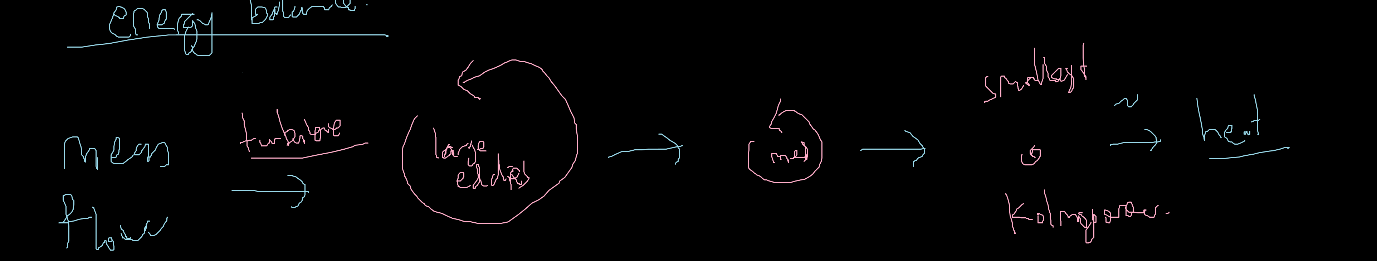
\includegraphics[width=6.26in,height=1.19in]{./media/image1.png}
	\end{Center}
\end{figure}


%%%%%%%%%%%%%%%%%%%% Figure/Image No: 1 Ends here %%%%%%%%%%%%%%%%%%%%

\par


\vspace{\baselineskip}
Kinetic energy (mean flow)  kinetic energy in turbulence (largest eddy)\par

 \[ rate of KE input \sim \frac{k}{t}=\frac{\frac{1}{2}u_{mean}^{2}}{t} \] \par

What is the timescale?\par

 \[ t \sim \frac{l}{u_{mean}} \] \par

L is characteristic length scale of largest eddy, usually comparable to pipe length, or if flow over a sphere, sphere diameter. \(  \)  \[ rate of KE input \sim \frac{k}{t}=\frac{\frac{1}{2}u_{mean}^{2}}{\frac{l}{u_{mean}}} \] \par

 \[ rate of KE input \sim \frac{k}{t}=\frac{\frac{1}{2}u_{mean}^{3}}{l} \] \par


\vspace{\baselineskip}
We also have KE dissipation,\par

 \[  \epsilon =rate of KE dissipation \sim \frac{k}{t} \] \par

We say that\par

 \[ k=\frac{1}{2}u_{smallest}^{2} \] \par

This is velocity scale of smallest eddy, defined by characteristic time and length scale.\par

Let’s call the legnthscale  \(  \eta  \) , timescale  \(  \tau_{ \eta } \) ,  \( u_{smallest}=u_{ \eta } \) \par


\vspace{\baselineskip}
What’s the timescale we are talking about for dissipation?\par

Timescale here is determined by kinematic viscosity\par

 \[  \nu   \left[ \frac{m^{2}}{s} \right]  \] \par

Now to make up for the units, we need an appropriate length scale:\par

 \[  \tau_{ \eta }=\frac{ \eta ^{2}}{ \nu } \] \par

Thus, this becomes our timescale.\par

Kinetic energy becomes\par

 \[ k=\frac{1}{2}u_{ \eta }^{2} \] \par

 \[  \epsilon  \sim \frac{k}{t}=\frac{u_{ \eta }^{2}}{ \tau_{ \eta }} \] \par

 \[  \epsilon  \sim \frac{k}{t}=\frac{u_{ \eta }^{2}}{\frac{ \eta ^{2}}{ \nu }} \] \par

 \[  \epsilon  \sim  \nu \frac{u_{ \eta }^{2}}{ \eta ^{2}} \] \par

All right that’s a lot of variables$ \ldots $  what use is it to us? We know  \(  \nu  \)  , for  \(  \epsilon  \)  we can scale\par

Rate of energy addition = Rate of energy dissipation\par

 \[  \epsilon  \sim \frac{u_{mean}^{3}}{l} \] \par

So those are based on \uline{macroscopic} properties\par

So  \(  \nu  \)  and  \(  \epsilon  \)  can be scaled based on macroscopic properties. We can find out the velocity, length and time scales based on these.\par

So let’s do length scale first:\par

 \[  \epsilon  \sim  \nu \frac{u_{ \eta }^{2}}{ \eta ^{2}} \] \par

We make a reasonable assumption\par

 \[ Re \sim 1 \] \par

 \[ Re=\frac{u_{ \eta } \eta }{ \nu } \] \par

This means\par

 \[  \nu  \sim u_{ \eta } \eta  \] \par

Or\par

 \[ u_{ \eta } \sim \frac{ \nu }{ \eta } \] \par


\vspace{\baselineskip}
 \[  \epsilon  \sim  \nu \frac{ \left( \frac{ \nu }{ \eta } \right) ^{2}}{ \eta ^{2}} \] \par

 \[  \epsilon  \sim \frac{ \nu ^{3}}{ \eta ^{4}} \] \par

 \[  \eta  \sim  \left( \frac{ \nu ^{3}}{ \epsilon } \right) ^{\frac{1}{4}} \] \par

This is known as the Kolmogorov scale$ \ldots $ \par

We can do the same for velocity\par

 \[ u_{ \eta } \sim \frac{ \nu }{ \eta }=\frac{ \nu }{ \left( \frac{ \nu ^{3}}{ \epsilon } \right) ^{\frac{1}{4}}}= \left(  \epsilon  \nu  \right) ^{\frac{1}{4}} \] \par

 \[  \tau_{ \eta }=\frac{ \eta }{u_{ \eta }}=\frac{ \left( \frac{ \nu ^{3}}{ \epsilon } \right) ^{\frac{1}{4}}}{ \left(  \epsilon  \nu  \right) ^{\frac{1}{4}}}= \left( \frac{ \nu }{ \epsilon } \right) ^{\frac{1}{2}} \] \par

Ok great, but let’s make it convenient for ourselves, scale it with Reynold’s number\par

 \[  \epsilon  \sim \frac{u_{mean}^{3}}{l} \] \par

Let’s do it for length scale first:\par

 \[  \eta  \sim  \left( \frac{ \nu ^{3}}{ \epsilon } \right) ^{\frac{1}{4}} \] \par

 \[  \eta  \sim  \left( \frac{ \nu ^{3}}{\frac{u_{mean}^{3}}{l}} \right) ^{\frac{1}{4}} \] \par

We can say  \( Re=\frac{u_{mean}l}{ \nu } \) \par


\vspace{\baselineskip}
So let’s make the inside look more favourable$ \ldots $ \par

 \[  \eta  \sim  \left( \frac{ \nu ^{3}}{\frac{u_{mean}^{3}l^{3}}{l^{4}}} \right) ^{\frac{1}{4}} \] \par


\vspace{\baselineskip}
 \[  \eta  \sim  \left( \frac{ \nu ^{3}}{u_{mean}^{3}l^{3}} \right) ^{\frac{1}{4}}l \] \par

 \[  \eta  \sim  \left( \frac{1}{Re^{3}} \right) ^{\frac{1}{4}}l \] \par

 \[ \frac{ \eta }{l} \sim Re^{-\frac{3}{4}} \] \par

Do the same for the rest and we find:\par

 \[ \frac{u_{ \eta }}{u_{0}} \sim Re^{-\frac{1}{4}} \] \par

 \[ \frac{ \tau_{ \eta }}{ \tau_{0}} \sim Re^{-\frac{1}{2}} \] \par

note that we can estimate the number of cells needed based on this:\par

no. of cells =  \( \frac{V_{total}}{V_{Cell}} \) \par

 \[ V_{cell} \sim  \eta ^{3} \] \par

 \[ V_{total} \sim l^{3} \] \par

 \[ n_{cells} \sim \frac{l^{3}}{ \eta ^{3}}=Re^{\frac{9}{4}} \] \par


\vspace{\baselineskip}
Hence for DNS, in free shear region, this usually means:\par

 \[ \frac{ \eta }{l} \sim Re^{-\frac{3}{4}} \] \par

So let’s say u have a 1m ish domain,\par

Re=10,000\par

Whats  \( o \left(  \eta  \right) ? \) \par

 \[  \eta  \sim 1m\ast \left( 10000 \right) ^{-\frac{3}{4}}=0.001 m or 1mm \] \par

What about if Re is 2000 (remember this is transistion!)\par

 \[  \eta  \sim 1m\ast \left( 2000 \right) ^{-\frac{3}{4}}=0.00334m  \left( 3mm \right)  \] \par

Of course, this  \(  \eta   \)  depends on the domain size$ \ldots $ \par


\vspace{\baselineskip}

\subsection{For scales closer to the wall, you need to pay more attention.}
Good rule of thumb (\cite{Komen2014}) :\par 

In wall normal direction:  \(  \Delta y^{+} \sim 0.05-0.5 \) \par

In wall parallel direction:  \(  \Delta z^{+}, \Delta x^{+} \sim 5 \) \par

 \[  \Delta y^{+}=\frac{ \Delta yu_{ \tau}}{ \nu } \] \par

Now that we know the standard DNS scales, we can look to LES and RANS for reference:\par


\vspace{\baselineskip}
Always make sure CFL is less than 1 for best results (stability)\par


\vspace{\baselineskip}
\section{LES grid sizing}\par

Note in the PL-DDES paper for comparison in direction perpendicular to wall,  \(  \Delta y^{+}=0.5 \) , equidistant for mixed convection,  \(  \Delta x^{+}=40 \) ,  \(  \Delta z^{+}=20 \) , is typical of LES grids (\cite{Ding2020}).\par

Usually for forced flows, BL =  \(  \delta  \)  ,  \(  \Delta x^{+} \approx \frac{1}{10} \delta  \) \par

(\cite{Spalart2006})\par

 \(  \delta  \rightarrow y^{+}=500 \)  (\cite{Tu2018})\par


\vspace{\baselineskip}
Shishkina, O., $\&$  Wagner, C. (2012). A numerical study of turbulent mixed convection in an enclosure with heated rectangular elements. Journal of Turbulence, (13), N22.\par


\vspace{\baselineskip}
\href{https://www.tandfonline.com/doi/full/10.1080/14685248.2012.677541?casa_token=3jNH8Q70aHwAAAAA%3AKCPlWHeKeQh13yrLYTQhy6HG-gZzr99FjKTvuij3VwOeD0kvTX13cLf9lY3Ezc8oBTgCz2e29pwvuQ}{https://www.tandfonline.com/doi/full/10.1080/14685248.2012.677541?casa\_token=3jNH8Q70aHwAAAAA$\%$ 3AKCPlWHeKeQh13yrLYTQhy6HG-gZzr99FjKTvuij3VwOeD0kvTX13cLf9lY3Ezc8oBTgCz2e29pwvuQ}\par


\vspace{\baselineskip}
Looking at this, a safe estimate is that les grid size is about 10x Kolmogorov length scale. \par


\vspace{\baselineskip}
\subsection{Wall functions (RANS)}\par

We generally have wall functions in the log law region  \( y^{+}>5 \) . Hence first mesh point should be in order of  \( y^{+}>5 \)  (\cite{Tu2018}). Usually  \( y^{+} \)  from 20 to 30 will do as a first start point, and have 8-10 mesh points in turb BL ( \( y^{+} \)  up to 500 ish) (\cite{Tu2018}). \par

Can check if mesh is fine enough by refining mesh and comparing plotting  \(  \nu _{t} \)  to  \(  \nu  \)  in BL. If no change then ok, only works for RANS though.\par

What about in parallel directions? (\cite{Spalart2006})\par

Usually in parallel direction for RANS, the parallel spacing would exceed the boundary layer thickness. \par

And this thickness is about  \( y^{+}=500 \) \par

So typical spacing in  \(  \Delta x^{+},~ \Delta z^{+} \)  direction would be 500 and up.\par

\par

\subsection{No Wall functions (low Re RANS)}\par

First mesh point at  \( y^{+}<1 \) , 5-10 nodal points from first point to  \( y^{+}=20 \) . Another 20-50 points in turbulent BL ( \( y^{+} \)  from 20 to $ \sim $ 500ish??) for total of 30-60 mesh points in BL for adequate mesh resolution without wall function.\par


\vspace{\baselineskip}
We can see from this order of magnitude estimate:\par

 \[  \Delta y^{+} \sim 50 \] \par

Whereas for DNS  \(  \Delta y^{+} \sim 0.05-0.5 \) \par

So this means RANS mesh length is about 100-1000 times bigger than Kolmogorov length scale.\par

In free shear region for Re $ \sim $  10000,  \( l \sim 1m \) \par

 \[  \eta  \sim l\ast{Re}^{-\frac{3}{4}} \] 

 \[  \eta  \sim 0.001m \] 

 \[ l_{RANS}=100\ast \eta =0.1 m \] 

This is just a rule of thumb. But should yield good result.\par

\section{Natural convection}\par

\href{http://thermopedia.com/content/1076/}{http://thermopedia.com/content/1076/}\par

\href{https://en.wikipedia.org/wiki/Rayleigh_number}{https://en.wikipedia.org/wiki/Rayleigh\_number}\par

Scheel, J. D., Emran, M. S., $\&$  Schumacher, J. (2013). Resolving the fine-scale structure in turbulent \textbf{\uline{Rayleigh–Bénard convection}}. New Journal of Physics, 15(11), 113063.\par

Perry, R. H., $\&$  Green, D. W. (2015). Perry’s chemical engineers’ handbook. \textit{Mc Graw}.\par


\vspace{\baselineskip}

\vspace{\baselineskip}
\subsection{Rayleigh–Bénard convection:}\par



%%%%%%%%%%%%%%%%%%%% Figure/Image No: 2 starts here %%%%%%%%%%%%%%%%%%%%

\begin{figure}[H]
	\begin{Center}
		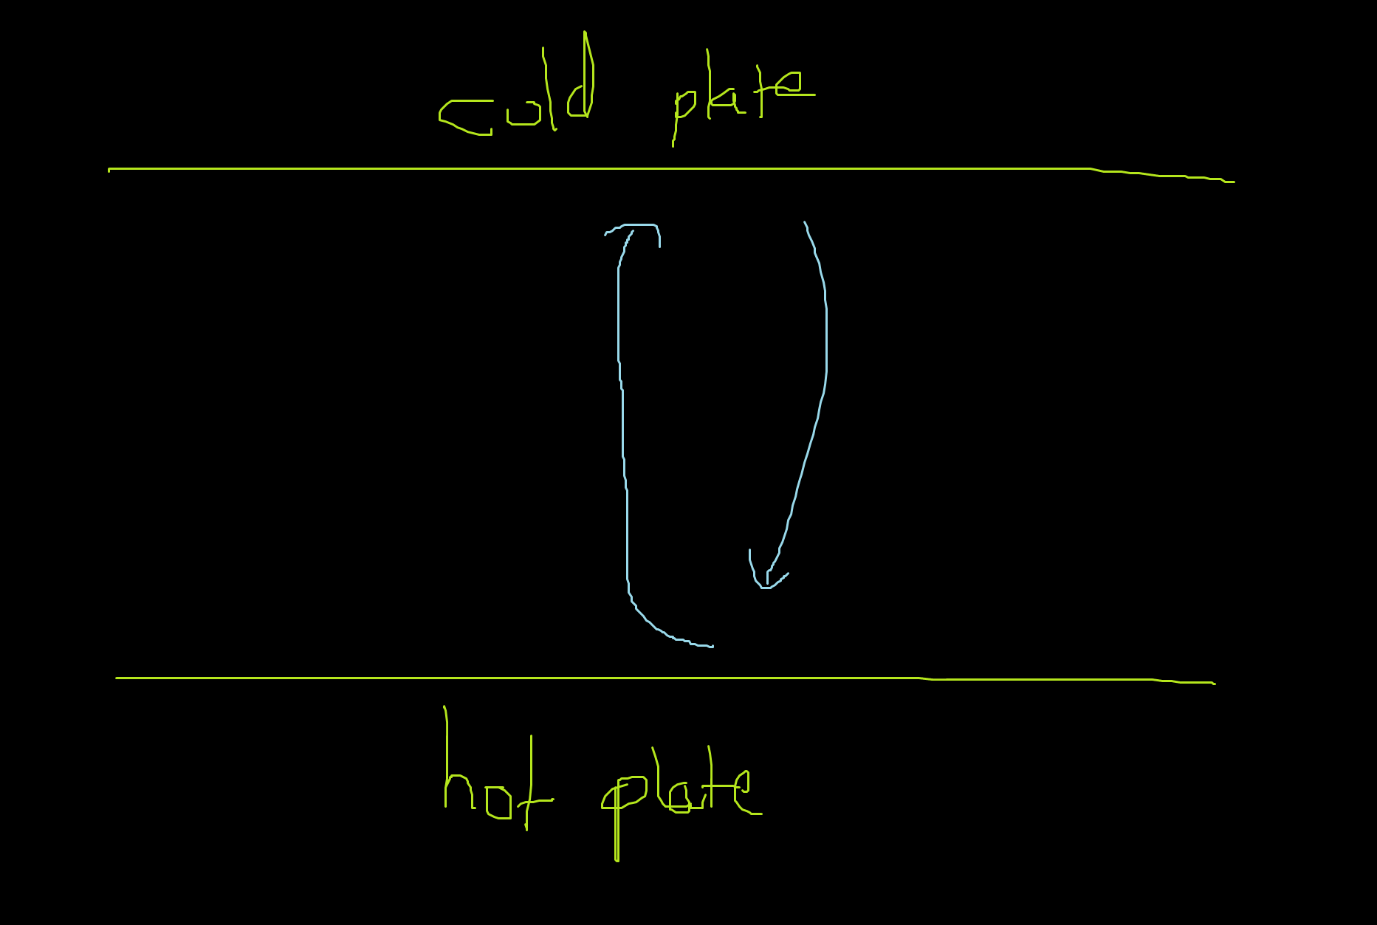
\includegraphics[width=6.26in,height=4.2in]{./media/image3.png}
	\end{Center}
\end{figure}


%%%%%%%%%%%%%%%%%%%% Figure/Image No: 2 Ends here %%%%%%%%%%%%%%%%%%%%

\par

Recall for forced flows:\par

 \[ \frac{ \eta }{l} \sim  \left( \frac{ \nu ^{3}}{ \epsilon } \right) ^{\frac{1}{4}} \] \par



%%%%%%%%%%%%%%%%%%%% Figure/Image No: 3 starts here %%%%%%%%%%%%%%%%%%%%

\begin{figure}[H]
	\begin{Center}
		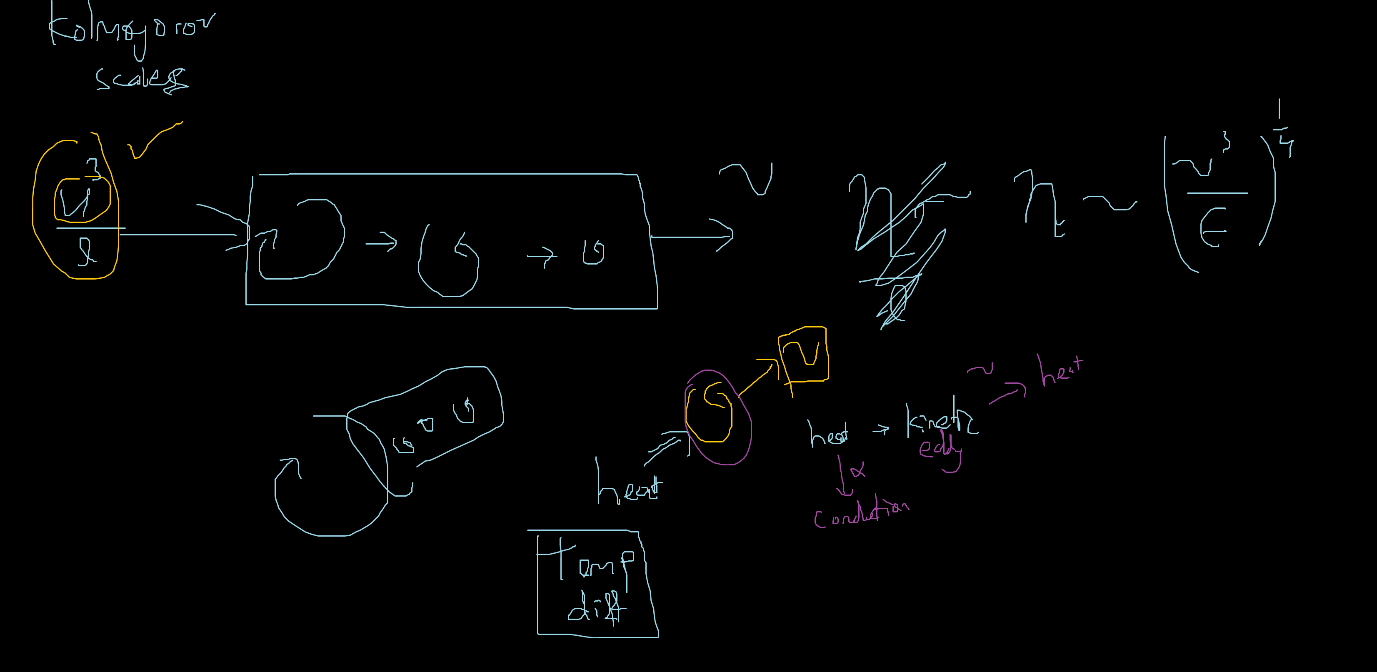
\includegraphics[width=6.26in,height=3.06in]{./media/image4.png}
	\end{Center}
\end{figure}


%%%%%%%%%%%%%%%%%%%% Figure/Image No: 3 Ends here %%%%%%%%%%%%%%%%%%%%

\par

For natural convection, the story is different$ \ldots $ \par

	\item In the smallest eddies, have two dissipation mechanisms now: \par

\begin{itemize}
	\item  \(  \alpha  \)  thermal conduction\par

	\item  \(  \nu  \)   viscous dissipation \par

	\item No eddy diffusivity or eddy heat flux to dissipate smallest eddies\par
\end{itemize}
\end{itemize}
This also means there are two types scales now involved, the Kolmogorov scale ( \(  \nu  \)  based dissipation), and the Batchelor scale ( \(  \alpha  \)  based dissipation).\par

 \[  \eta _{B}=\frac{ \eta _{kolmogorov}}{\sqrt[]{Pr}} \] \par

For large Pr, batchelor scale dominates.(\cite{Scheel2013})\par

\subsubsection{Kolmogorov Scale(\cite{Scheel2013})}\par

 \[ \frac{ \eta }{l} \sim  \left( \frac{ \nu ^{3}}{ \epsilon } \right) ^{\frac{1}{4}} \] \par

Skipping derivation, but we nondimensionalize  \(  \epsilon  \)  to get:\par

Also apply characteristic length l=H (cell height) \par

 \[ \frac{ \eta _{k}}{H}=\frac{Pr^{\frac{3}{8}}}{Ra^{\frac{3}{8}}}\frac{1}{\widetilde{ \epsilon }^{\frac{1}{4}}} \] \par

Note: \( ~\widetilde{ \epsilon }^{\frac{1}{4}} \)  is dimensionless\par

On average,\par

 \[ \widetilde{ \langle  \epsilon  \rangle }=\frac{Nu}{\sqrt[]{RaPr}} \] \par

 \[ \frac{ \eta _{k}}{H}= \left( \frac{Pr^{2}}{ \left( Nu-1 \right) Ra} \right) ^{\frac{1}{4}} \] \par

Evaluate dimensionless numbers (fluid properties) at  \( T_{film}=\frac{T_{S}+T_{\infty}}{2} \) \par

\subsubsection{Batchelor scale (\cite{Scheel2013}):}\par

 \[  \eta _{B}=\frac{ \eta _{k}}{\sqrt[]{Pr}} \] \par

 \[ \frac{ \eta _{B}}{H}=\frac{Pr^{\frac{1}{8}}}{Ra^{\frac{3}{8}}}\frac{1}{\widetilde{ \epsilon }^{\frac{1}{4}}} \] \par

 \[ \frac{ \eta _{B}}{H}= \left( \frac{1}{ \left( Nu-1 \right) Ra} \right) ^{\frac{1}{4}} \] \par

As to which is smaller depends on Pr\par

 \[ \frac{ \eta _{k}}{H}= \left( \frac{Pr^{2}}{ \left( Nu-1 \right) Ra} \right) ^{\frac{1}{4}};~\frac{ \eta _{B}}{H}= \left( \frac{1}{ \left( Nu-1 \right) Ra} \right) ^{\frac{1}{4}} \] \par


\vspace{\baselineskip}
For large Pr, batchelor scale is smaller.\par

For small Pr, Kolmogorov scale is smaller.\par


\vspace{\baselineskip}
Pre-requisite: need to know Nu, Pr and Ra in order to know the length scale size$ \ldots $ \par

Also note, these scales are for natural convection, which is \uline{near the wall} anyhow. Estimates with wall function aren’t as necessary.\par


\vspace{\baselineskip}
A rough scaling for  \( Nu \) : like Re, it depends on the situation.\par

Eg. Flat plate flow, high Pr (\cite{Bejan2013})\par

 \[ Nu \sim Ra_{H}^{\frac{1}{3}} \] \par

For Rayleigh Benard convection (\cite{Perry2015})\par

 \[ Nu=Ra_{H}^{\frac{1}{3}} \] \par


\vspace{\baselineskip}

\vspace{\baselineskip}
\section{Mixed convection (free shear)}\par

Just an estimate:\par

Three scales we discussed:\par

 \[ \frac{ \eta }{l} \sim Re^{-\frac{3}{4}} \] \par

 \[ \frac{ \eta _{B}}{H}= \left( \frac{1}{ \left( Nu-1 \right) Ra} \right) ^{\frac{1}{4}} \] \par

 \[ \frac{ \eta _{k}}{H}= \left( \frac{Pr^{2}}{ \left( Nu-1 \right) Ra} \right) ^{\frac{1}{4}} \] \par

You could pick the smallest of the three to start$ \ldots $ \par


(25 June 2020) Note that Batchelor scales are also important in forced convection, forgot to add this. $\eta_{B}=\frac{\eta_{k}}{\sqrt{Pr}}$ Please take note.




\vspace{\baselineskip}
\uline{In literature, most mesh sizes are listed in terms of wall scale}\par

 \[ Ri=\frac{Gr}{Re^{2}} \] \par

In literature:\par

Base your grid spacing on wall spacing estimates (done in literature) (\cite{You2003} )\par

Eg. For a tube:\par

 \[ 0.17 \leq  \Delta r^{+} \leq 5.1 \] \par

 \[  \Delta  \phi ^{+} \approx 8.85 \] \par

 \[ 7 \leq  \Delta x^{+} \leq 10.5 \] \par

These are basically  \( r, \theta ,z \)  coordinates.\par

But it gives you an idea of the grid spacing needed!\par


\vspace{\baselineskip}

\vspace{\baselineskip}

\section{Friction Velocity Estimates for Forced and Natural Flows}
\addcontentsline{toc}{section}{Friction Velocity Estimates for Forced and Natural Flows}

\vspace{\baselineskip}
U need wall shear stress to predict friction velocity:\par

 \[ u_{ \tau}=\sqrt[]{\frac{ \tau_{wall}}{ \rho }} \] \par

 \[ y^{+}=\frac{yu_{ \tau}}{ \nu } \] \par

Standard pipe correlations (moody chart predicting Fanning’s friction factor)\par

 \[ f=\frac{ \tau_{wall}}{\frac{1}{2} \rho u_{mean}^{2}} \] \par

From Churchill (in perry’s chemical engineering handbook) (\cite{Perry2015})\par

 \[ \frac{1}{\sqrt[]{f}}=-4\log _{10} \left( 0.27\frac{ \epsilon }{D}+ \left( \frac{7}{Re_{mean}} \right) ^{0.9} \right)  \] \par

For smooth pipes, surface roughness =0 (for most DNS we ignore this anyhow)\par

Check whether it’s  \( \ln x~or\log _{10}x \) ?\par

Quick calculation:\par

 \[ Re_{mean}=5,000 \] \par

 \[ Re=\frac{uD}{ \nu } \] \par

From graph:  \( f \approx 0.0091 \) \par

Excel calculated value\par

 \[ \frac{1}{\sqrt[]{f}}=-4\log _{10} \left(  \left( \frac{7}{5000} \right) ^{0.9} \right) =10.2739 \] \par

 \[ f= \left( \frac{1}{10.2739} \right) ^{2}=0.00947384 \] \par


\vspace{\baselineskip}
Good match!\par

Can we correlate  \( Re_{mean} \)  to  \( u_{ \tau} \)  for smooth pipes?\par

Absolutely!!\par

 \[ f=\frac{ \tau_{wall}}{\frac{1}{2} \rho u_{mean}^{2}} \] \par

 \[ u_{ \tau}=\sqrt[]{\frac{ \tau_{wall}}{ \rho }} \] \par

 \[ u_{ \tau}=\sqrt[]{\frac{\frac{1}{2} \rho u_{mean}^{2}f}{ \rho }} \] \par

 \[ u_{ \tau}=\sqrt[]{\frac{1}{2}u_{mean}^{2}f} \] \par

 \[ u_{ \tau}=u_{mean}\sqrt[]{\frac{1}{2}f} \] \par

Noting:\par

 \[ \frac{1}{\sqrt[]{f}}=-4\log _{10} \left( 0.27\frac{ \epsilon }{D}+ \left( \frac{7}{Re_{mean}} \right) ^{0.9} \right)  \] \par

Tada!!\par


\vspace{\baselineskip}
 \[ u_{ \tau}=u_{mean}\sqrt[]{\frac{1}{2}}\ast\frac{1}{-4\log _{10} \left( 0.27\frac{ \epsilon }{D}+ \left( \frac{7}{Re_{mean}} \right) ^{0.9} \right) } \] \par


\vspace{\baselineskip}
And if we want to correlate  \( Re_{ \tau} \)  in terms of  \( Re_{mean} \) \par

Provided length scale is the same, (which is should be)\par

 \[ \frac{u_{ \tau}L}{ \nu }=\frac{u_{mean}L}{ \nu }\sqrt[]{\frac{1}{2}}\ast\frac{1}{-4\log _{10} \left( 0.27\frac{ \epsilon }{D}+ \left( \frac{7}{Re_{mean}} \right) ^{0.9} \right) } \] \par

If L=D (pipe diameter)\par

Then we define: \par

 \[ Re_{ \tau}=\frac{u_{ \tau}D}{ \nu } \] \par

Tada!!\par

 \[ Re_{ \tau}=Re_{mean}~\sqrt[]{\frac{1}{2}}\ast\frac{1}{-4\log _{10} \left( 0.27\frac{ \epsilon }{D}+ \left( \frac{7}{Re_{mean}} \right) ^{0.9} \right) } \] \par

Okay if we don’t want to remember logarithm and everything$ \ldots $  and simplify for smooth pipes:\par

 \[ Re_{ \tau}=Re_{mean}~\sqrt[]{\frac{1}{2}}\ast\frac{1}{-4\log _{10} \left(  \left( \frac{7}{Re_{mean}} \right) ^{0.9} \right) } \] \par

Plot in excel$ \ldots $ \par

Again you have to be \uline{careful} what length scale you are talking about before u use this formula!!!\par



%%%%%%%%%%%%%%%%%%%% Figure/Image No: 4 starts here %%%%%%%%%%%%%%%%%%%%

\begin{figure}[H]
	\begin{Center}
		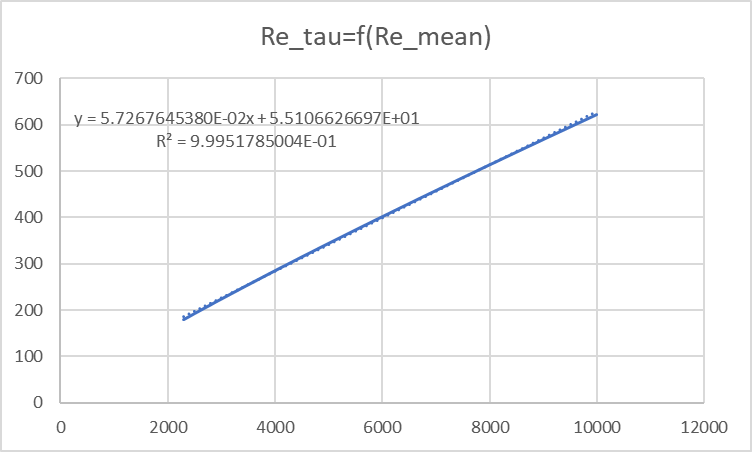
\includegraphics[width=5.01in,height=3.01in]{./media/image5.png}
	\end{Center}
\end{figure}


%%%%%%%%%%%%%%%%%%%% Figure/Image No: 4 Ends here %%%%%%%%%%%%%%%%%%%%

\par

 \[ Re_{ \tau}=5.72676\ast10^{-2}\ast{Re}_{mean}+5.51066 \] \par

(5 d.p)\par

This is a linear graph for \uline{smooth} pipes, so u can get  \( Re_{ \tau} \)  and  \( u_{ \tau} \)  estimate for DNS data$ \ldots $ \par

So what is  \( x^{+}? \) \par

 \[ x^{+}=\frac{xu_{ \tau}}{ \nu } \] \par

But \par

 \[ Re_{ \tau}=\frac{u_{ \tau}L}{ \nu } \] \par

We can write in this manner:\par

 \[ x^{+}=x\ast\frac{Re_{ \tau}}{L} \] \par

Very simple formula if you know your  \( Re_{ \tau} \)  beforehand.\par

So let’s say we have  \( Re_{ \tau}=180 \)  (corresponds to  \( Re_{mean} \approx 2300 \) )\par

What is the how small should your DNS mesh be for 0.1m diameter pipe?\par

  \(  \Delta x^{+} \approx 0.05  \left( smallest DNS mesh \right)  \) \par

 \[ x=\frac{1}{\frac{{Re}_{ \tau}}{L}}\ast{x}^{+} \] \par

 \[ x=\frac{1}{\frac{180}{0.1}}\ast0.05=2.777\ast10^{-5}m=0.02777 mm \] \par


\vspace{\baselineskip}
We are talking in microns here!\par

So small$ \ldots $ \par

And how thick is the VSL region?\par

 \[ x^{+} \approx 5 \] \par

  \(  \)  \[ x=\frac{1}{\frac{180}{0.1}}\ast5=2.777\ast10^{-3}m \approx 2.777 mm \] \par

That’s quite thin!\par

And the BL thickness estimate?  \( x^{+}~or~y^{+}=500 \) \par

 \[ x=\frac{1}{\frac{180}{0.1}}\ast500=2.777\ast10^{-1}m \approx 27.8 cm \] \par

That’s where we get it!\par


\vspace{\baselineskip}
How does  \(  \Delta x^{+} \)  compare to Kolmogorov scale?  \( Re_{mean} \approx 2300 \) \par

 \[ \frac{ \eta }{D} \sim \frac{1}{Re_{mean}^{\frac{3}{4}}}=0.003010954  \] \par


\vspace{\baselineskip}
 \[  \eta  \sim \frac{1}{Re_{mean}^{\frac{3}{4}}}\ast0.1m=0.003010954\ast0.1m=0.3mm \] \par


\vspace{\baselineskip}
Kolmogorov lengthscale about 10x smaller (1 order of magnitude smaller) than VSL region! \par

It’s about 10x bigger than the smallest DNS mesh size.\par


\vspace{\baselineskip}
In other words, kolmmogorov lengthscale is about \par

 \[  \eta  \approx  \Delta x^{+}\ast\frac{L}{Re_{ \tau}} \] \par

 \[  \Delta x^{+} \approx 1.85 \] \par

This is for this case only, or in general \uline{low Re DNS with smooth pipe}, but we can see the rough relationship here$ \ldots $ \par


\vspace{\baselineskip}
For mixed convection of low Richardson number, this rule should still apply.\par

\section{Near Wall Smallest Scale Estimates for Natural Convection}
\addcontentsline{toc}{section}{Near Wall Smallest Scale Estimates for Natural Convection}
Ampofo, F., $\&$  Karayiannis, T. G. (2003). Experimental benchmark data for turbulent natural convection in an air filled square cavity. International Journal of Heat and Mass Transfer, 46(19), 3551–3572. https://doi.org/https://doi.org/10.1016/S0017-9310(03)00147-9\par


\vspace{\baselineskip}
Hardcore estimate (\cite{Yuan1993}):\par



%%%%%%%%%%%%%%%%%%%% Table No: 1 starts here %%%%%%%%%%%%%%%%%%%%


\begin{table}[H]
 			\centering
\begin{tabular}{p{1.89in}p{1.89in}p{1.89in}}
\hline
%row no:1
\multicolumn{1}{|p{1.89in}}{} & 
\multicolumn{1}{|p{1.89in}}{Forced Convection} & 
\multicolumn{1}{|p{1.89in}|}{Natural Convection} \\
\hhline{---}
%row no:2
\multicolumn{1}{|p{1.89in}}{Distance from wall} & 
\multicolumn{1}{|p{1.89in}}{ \( y^{+} \equiv \frac{yu_{ \tau}}{ \nu } \) } & 
\multicolumn{1}{|p{1.89in}|}{ \( y^{\ast} \equiv \frac{yu_{q}}{ \alpha } \) } \\
\hhline{---}
%row no:3
\multicolumn{1}{|p{1.89in}}{Velocity} & 
\multicolumn{1}{|p{1.89in}}{ \( u^{+} \equiv \frac{u}{u_{ \tau}} \) } & 
\multicolumn{1}{|p{1.89in}|}{ \( u^{\ast\ast} \equiv \frac{u_{q}^{3}u}{u_{ \tau}^{4}} \) } \\
\hhline{---}
%row no:4
\multicolumn{1}{|p{1.89in}}{Temperature} & 
\multicolumn{1}{|p{1.89in}}{ \( T^{+} \equiv \frac{ \left( T_{wall}-T \right) u_{ \tau}}{ \left( \frac{q_{wall}}{ \rho c_{p}} \right) } \) } & 
\multicolumn{1}{|p{1.89in}|}{ \( T_{natl}^{\ast} \equiv \frac{ \left( T_{wall}-T \right) }{T_{q}} \) } \\
\hhline{---}
%row no:5
\multicolumn{1}{|p{1.89in}}{Reference dimensionless quantities} & 
\multicolumn{1}{|p{1.89in}}{ \( u_{ \tau} \equiv \sqrt[]{\frac{ \tau_{wall}}{ \rho }} \) } & 
\multicolumn{1}{|p{1.89in}|}{ \( u_{q} \equiv  \left( \frac{g \beta  \alpha q_{wall}}{ \rho c_{P}} \right) ^{\frac{1}{4}}~ \)  \par  \( T_{q} \equiv  \left( \frac{q_{wall}^{3}}{g \beta  \alpha  \left(  \rho c_{p} \right) ^{3}} \right) ^{\frac{1}{4}} \) } \\
\hhline{---}

\end{tabular}
 \end{table}


%%%%%%%%%%%%%%%%%%%% Table No: 1 ends here %%%%%%%%%%%%%%%%%%%%


\vspace{\baselineskip}
 \[ u_{q} \equiv  \left( \frac{g \beta  \alpha q_{wall}}{ \rho c_{P}} \right) ^{\frac{1}{4}} \] \par

Temperature length scales\par

 \[ y^{\ast} \equiv \frac{yu_{q}}{ \alpha } \] \par

Velocity length scales\par

 \[ y_{1}^{\ast\ast}=\frac{yu_{q}^{3}}{ \alpha u_{ \tau}^{2}}=y^{\ast}\frac{u_{q}^{2}}{u_{ \tau}^{2}} \] \par

Problem: Estimating  \( u_{ \tau} \)  is a pain (correlations are sparse if anything – most people don’t care much for wall shear stress in natural convection applications)\par


\vspace{\baselineskip}
\subsection{Ballpark Estimate:}\par

\begin{itemize}
	\item 10x smaller than smallest of Kolmogorov/Batchelor scales\par

	\item  \( \frac{ \eta }{l} \sim Re^{-\frac{3}{4}} \) \par

	\item  \( \frac{ \eta _{B}}{H}= \left( \frac{1}{ \left( Nu-1 \right) Ra} \right) ^{\frac{1}{4}} \) \par

	\item  \( \frac{ \eta _{k}}{H}= \left( \frac{Pr^{2}}{ \left( Nu-1 \right) Ra} \right) ^{\frac{1}{4}} \) \par


\vspace{\baselineskip}
Lower Bound estimate  convert natural convection into mixed convection (cheating):\par
\end{itemize}

\subsection{Method 1: Pretend the situation is a mixed convection, set Richardson number to 0.1} \par

\begin{itemize}
	\item Ie  \( \frac{Gr}{Re^{2}}=0.1 \) \par

	\item  \( Re=\sqrt[]{10Gr} \) \par

	\item  \( \sqrt[]{10Gr}=\frac{u_{buoyancy}L}{ \nu } \) \par


\end{itemize}

\subsection{ Method 2: use buoyancy Velocity to estimate  \( C_{f} \) }\par

\begin{itemize}
	\item Ie  \( Gr=Re^{2} \) \par

	\item  \( \sqrt[]{Gr}=\frac{u_{buoyancy}L}{ \nu } \) \par

\end{itemize}
\vspace{\baselineskip}

\vspace{\baselineskip}

\vspace{\baselineskip}
Eg. Square cavity\par



%%%%%%%%%%%%%%%%%%%% Figure/Image No: 5 starts here %%%%%%%%%%%%%%%%%%%%

\begin{figure}[H]
	\begin{Center}
		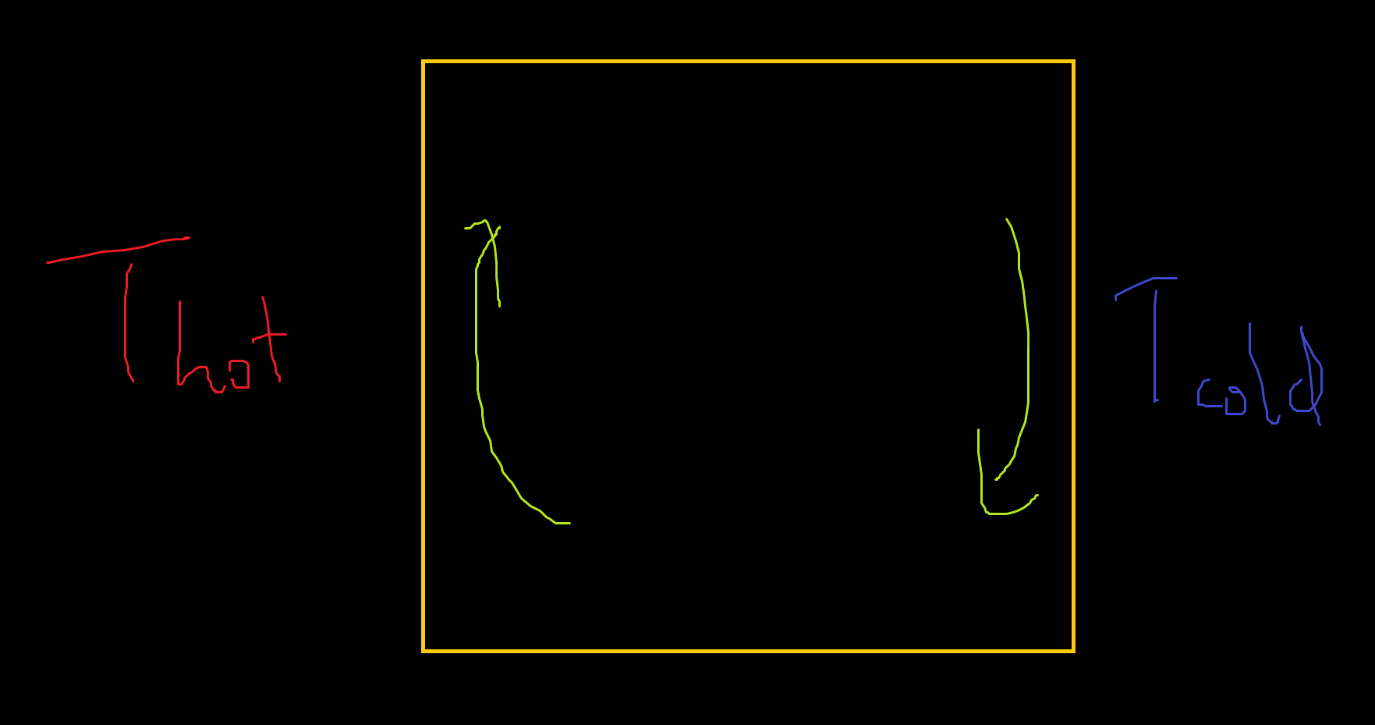
\includegraphics[width=6.26in,height=3.3in]{./media/image6.png}
	\end{Center}
\end{figure}


%%%%%%%%%%%%%%%%%%%% Figure/Image No: 5 Ends here %%%%%%%%%%%%%%%%%%%%

\par

How to estimate?\par

Let’s do it for airflow: simple example (\cite{Ampofo2003})\par

0.75\ $\ast$  0.75 $\ast$  1.5  (m\textsuperscript{3}) cavity\par

 \[ T_{hot}=50 ^{\circ}C  \] \par

 \[ T_{cold}=10 ^{\circ}C  \] \par

 \[ Ra=1.58\ast10^{9} \] \par

 \[ Ra=\frac{g \beta  \left( T_{hot}-T_{cold} \right) H^{3}}{ \nu ^{2}}Pr \] \par

 \[ Pr=0.71 \] \par

 \[ \frac{ \eta _{k}}{H}= \left( \frac{Pr^{2}}{ \left( Nu-1 \right) Ra} \right) ^{\frac{1}{4}} \] \par

Let’s estimate the Kolmogorov scale:\par

 \[ Nu \sim Ra_{H}^{\frac{1}{3}} \] \par

 \[ Nu=0.15\ast{Ra}_{H}^{\frac{1}{3}}~ \] \par

 \[ \frac{ \eta _{k}}{H}= \left( \frac{Pr^{2}}{ \left( Ra_{H}^{\frac{1}{3}}-1 \right) Ra} \right) ^{\frac{1}{4}}= \left( \frac{0.71^{2}}{ \left(  \left( 1.58\ast10^{9} \right) ^{\frac{1}{3}}-1 \right) 1.58\ast10^{9}} \right) ^{\frac{1}{4}} \] \par

Since  \( Ra_{H}^{\frac{1}{3}} \gg 1 \) \par

 \[ \frac{ \eta _{k}}{H}= \left( \frac{Pr^{2}}{ \left( Ra_{H}^{\frac{1}{3}}-1 \right) Ra} \right) ^{\frac{1}{4}}= \left( \frac{0.71^{2}}{ \left( 1.58\ast10^{9} \right) ^{\frac{4}{3}}} \right) ^{\frac{1}{4}} \approx 0.000723453 \] \par

If  \( H=0.75 \) \par

 \[  \eta _{K}=0.00054259 m \approx 0.5 mm \] \par

What about the Batchelor Scale?\par

 \[  \eta _{B}=\frac{ \eta _{K}}{\sqrt[]{Pr}}=0.000643935 m \approx 0.6 mm \] \par

Here, Kolmogorov scales are smaller\par


\vspace{\baselineskip}
Using minimum mesh size =1/10 of Kolmogorov/Batchelor scale,\par

 \[ smallest~ \Delta x \approx 0.05 mm  \left( wall normal \right)  \] \par


\vspace{\baselineskip}
\subsubsection{Worked Examples of Lower Bound Estimates:}\par

Method 1: Pretend the situation is a mixed convection, set Richardson number to 0.1\par

\begin{itemize}
	\item Ie  \( \frac{Gr}{Re^{2}}=0.1 \) \par

	\item  \( Re=\sqrt[]{10Gr} \) \par

	\item  \( \sqrt[]{10Gr}=\frac{u_{buoyancy}L}{ \nu } \) \par


\end{itemize}
Worked Example Method 2: use buoyancy Velocity to estimate  \( C_{f} \) \par

\begin{itemize}
	\item Ie  \( Gr=Re^{2} \) \par

	\item  \( \sqrt[]{Gr}=\frac{u_{buoyancy}L}{ \nu } \) \par
\end{itemize}

Schultz Grunow Correlation (\cite{Bejan2013}): \( C_{f,x}=0.37\ast \left\lbrace \log _{10} \left( \frac{U_{\infty}x}{ \nu } \right)  \right\rbrace ^{-2.584} \)

Id say substitute  \( Re_{x}=\frac{U_{\infty}x}{ \nu } \) \  as  \( Re_{x}=\sqrt[]{Gr} \)  (or  \( \sqrt[]{\text{10 Gr}} \) ) \par


\vspace{\baselineskip}
Compress the formula:\par

 \[ C_{f,x}=0.37\ast \left\lbrace \log _{10} \left( \sqrt[]{10Gr} \right)  \right\rbrace ^{-2.584} \] \par

 \[ C_{f,x}=0.37\ast \left\lbrace \log _{10} \left( \sqrt[]{Gr} \right)  \right\rbrace ^{-2.584} \] \par

Estimate for skin friction$ \ldots $ \par

We derived in the last video:\par

 \[ u_{ \tau}=u_{mean}\sqrt[]{\frac{1}{2}f} \] \par

Here, if the  \( L=H \)  for both sides, multiply, by  \( \frac{H}{ \nu } \) \par

 \[ Re_{ \tau}=Re_{mean}\sqrt[]{\frac{1}{2}f} \] \par

Substitute:\par

 \[ Re_{ \tau}=\sqrt[]{10Gr}\sqrt[]{\frac{1}{2}0.37\ast \left\lbrace \log _{10} \left( \sqrt[]{10Gr} \right)  \right\rbrace ^{-2.584}} \] \par

 \[ Re_{ \tau}=\sqrt[]{Gr}\sqrt[]{\frac{1}{2}0.37\ast \left\lbrace \log _{10} \left( \sqrt[]{Gr} \right)  \right\rbrace ^{-2.584}} \] \par

Here, \par

 \[ Ra=1.58\ast10^{9} \] \par

But Pr is  \( o \left( 1 \right)  \)  so  \( o \left( Ra \right) =o \left( Gr \right)  \) \par

If im just estimating order of magnitude, just substitute Ra in, otherwise of course, divide by Pr\par

This is quick and fast estimate\par

 \[ Re_{ \tau}=\sqrt[]{1.58\ast10^{10}}\sqrt[]{\frac{1}{2}0.37\ast \left\{ \log _{10} \left( \sqrt[]{1.58\ast10^{10}} \right)  \right\rbrace ^{-2.584}} \] \par

 \[ Re_{ \tau}=6588 \] \par

 \[ Re_{ \tau}=\sqrt[]{1.58\ast10^{9}}\sqrt[]{\frac{1}{2}0.37\ast \left\{ \log _{10} \left( \sqrt[]{1.58\ast10^{9}} \right)  \right\rbrace ^{-2.584}} \] \par

 \[ Re_{ \tau}=2380 \] \par

Looks like  \( Re_{ \tau} \)  is quite high! But this is ultraconservative anyhow\par

Now let’s estimate our length scale:\par

 \[ x= \Delta x^{+}\ast\frac{L}{Re_{ \tau}}=0.05\ast\frac{0.75}{6588}=5.69\ast10^{-6}m \approx 0.006 mm \] \par

(absolute smallest length scale, no smaller)\par

 \[ x= \Delta x^{+}\ast\frac{L}{Re_{ \tau}}=0.05\ast\frac{0.75}{2380}=1.57\ast10^{-5}m \approx 0.02 mm \] \par

We can see this estimate is on the same order of magnitude as 10x below Kolmogorov/Batchelor scale. Pretty good!\par

 \[  \eta _{K}=0.00054259 m \approx 0.5 mm \] \par

 \[  \eta _{B}=\frac{ \eta _{K}}{\sqrt[]{Pr}}=0.000643935 m \approx 0.6 mm \] \par


\vspace{\baselineskip}
Now let’s compare these with the hardcore estimates, and similar techniques see these scales:\par

Temperature length scales\par

 \[ y^{\ast} \equiv \frac{yu_{q}}{ \alpha } \] \par

Velocity length scales\par

 \[ y_{1}^{\ast\ast}=\frac{yu_{q}^{3}}{ \alpha u_{ \tau}^{2}}=y^{\ast}\frac{u_{q}^{2}}{u_{ \tau}^{2}} \] \par

 \[ u_{q} \equiv  \left( \frac{g \beta  \alpha q_{wall}}{ \rho c_{P}} \right) ^{\frac{1}{4}} \] \par

Let’s try to make look more like dimensionless numbers:\par

 \[ \frac{u_{q}}{ \alpha } \equiv \frac{1}{ \alpha } \left( \frac{g \beta  \alpha q_{wall}}{ \rho c_{P}} \right) ^{\frac{1}{4}} \] \par

 \[ Ra_{H}=\frac{g \beta  \left( T_{H}-T_{C} \right) H^{3}}{ \nu  \alpha } \] \par

 \[ g \beta = \nu  \alpha \frac{Ra_{H}}{ \left( T_{H}-T_{C} \right) H^{3}} \] \par

Substitute,\par

 \[ \frac{u_{q}}{ \alpha } \equiv \frac{1}{ \alpha } \left( \frac{ \nu  \alpha \frac{Ra_{H}}{ \left( T_{H}-T_{C} \right) H^{3}} \alpha q_{wall}}{ \rho c_{P}} \right) ^{\frac{1}{4}} \] \par

 \[ \frac{u_{q}}{ \alpha } \equiv \frac{1}{ \alpha } \left( \frac{ \nu  \alpha ^{2}Ra_{H}q_{wall}}{ \rho c_{P}H^{3} \left( T_{H}-T_{C} \right) } \right) ^{\frac{1}{4}} \] \par

What’s Nu?\par

 \[ Nu_{local}=\frac{hL}{k} \] \par

L=H (cavity height)\par


\vspace{\baselineskip}
 \[ h=\frac{q}{T_{h}-T_{c}} \] \par

 \[ Nu_{local}=\frac{q}{T_{h}-T_{c}}\frac{H}{k} \] \par

 \[ \frac{q}{T_{h}-T_{c}}=\frac{Nu_{local}k}{H} \] \par

Substitute!\par

 \[ \frac{u_{q}}{ \alpha } \equiv \frac{1}{ \alpha } \left( \frac{ \nu  \alpha ^{2}Ra_{H}q_{wall}}{ \rho c_{P}H^{3} \left( T_{H}-T_{C} \right) } \right) ^{\frac{1}{4}} \] \par

 \[ \frac{u_{q}}{ \alpha } \equiv \frac{1}{ \alpha } \left( \frac{ \nu  \alpha ^{2}Ra_{H}\frac{Nu_{local}k}{H}}{ \rho c_{P}H^{3}} \right) ^{\frac{1}{4}} \] \par

 \[ \frac{u_{q}}{ \alpha } \equiv \frac{1}{ \alpha } \left( \frac{ \nu  \alpha ^{2}Ra_{H}Nu_{local}k}{ \rho c_{P}H^{4}} \right) ^{\frac{1}{4}} \] \par

Substitute  \(  \alpha =\frac{k}{ \rho c_{p}} \) \par

 \[ \frac{u_{q}}{ \alpha } \equiv \frac{1}{ \alpha } \left( \frac{ \nu  \alpha ^{3}Ra_{H}Nu_{local}}{H^{4}} \right) ^{\frac{1}{4}} \] \par

And finally, we have  \( Pr \) \par

 \[  \nu = \alpha Pr \] \par

 \[ \frac{u_{q}}{ \alpha } \equiv \frac{1}{ \alpha } \left( \frac{ \alpha ^{4}P\text{r R}a_{H}Nu_{local}}{H^{4}} \right) ^{\frac{1}{4}} \] \par

 \[ \frac{u_{q}}{ \alpha } \equiv \frac{1}{ \alpha } \left( P\text{r R}a_{H}Nu_{local} \right) ^{\frac{1}{4}}\frac{ \alpha }{H} \] \par

 \[ \frac{u_{q}}{ \alpha } \equiv \frac{ \left( P\text{r R}a_{H}Nu_{local} \right) ^{\frac{1}{4}}}{H} \] \par

Or \par

 \[ u_{q}=\frac{ \alpha }{H} \left( P\text{r R}a_{H}Nu_{local} \right) ^{\frac{1}{4}} \] \par

This is much more palatable!\par

Let’s check out the thermal length scale:\par

 \[ y^{\ast} \equiv \frac{yu_{q}}{ \alpha } \] \par

 \[ y^{\ast} \equiv y\frac{ \left( P\text{r R}a_{H}Nu_{local} \right) ^{\frac{1}{4}}}{H} \] \par

 \[ y=y^{\ast}\frac{H}{ \left( P\text{r R}a_{H}Nu_{local} \right) ^{\frac{1}{4}}} \] \par

Assuming we want  \( y^{\ast} \approx 0.05 \) \par

 \[ y=0.05\frac{H}{ \left( P\text{r R}a_{H}Nu_{local} \right) ^{\frac{1}{4}}} \] \par


\vspace{\baselineskip}
Substitute  \( Nu \sim Ra_{H}^{\frac{1}{3}} \) \par

 \[ y=0.05\frac{H}{ \left( P\text{r R}a_{H}^{\frac{4}{3}} \right) ^{\frac{1}{4}}} \] \par

 \[ Ra=1.58\ast10^{9} \] \par

 \[ Pr=0.71 \] \par

 \[ H=0.75m \] \par

 \[ y_{thermal}=0.05\frac{0.75}{ \left( 0.71~ \left( 1.58e9 \right) ^{\frac{4}{3}} \right) ^{\frac{1}{4}}}=3.51\ast10^{-5}m \approx 0.035 mm! \] \par

About 10x below Batchelor scale too\par

Let’s test the momentum BL scales,\par

 \[ y_{1}^{\ast\ast}=\frac{yu_{q}^{3}}{ \alpha u_{ \tau}^{2}}=y^{\ast}\frac{u_{q}^{2}}{u_{ \tau}^{2}} \] \par

 \[  \Delta y^{\ast}=\frac{yu_{q}}{ \alpha }\frac{u_{q}^{2}}{u_{ \tau}^{2}} \] \par

Let’s make life easier and formulate  \(  \left( \frac{u_{q}}{u_{ \tau}} \right) ^{2} \)  in terms of dimensionless numbers\par

 \[ Re_{ \tau}=\frac{u_{ \tau}L}{ \nu } \] \par

 \[ u_{ \tau}=\frac{Re_{ \tau} \nu }{L} \] \par

And for  \( u_{q} \) ,\par


\vspace{\baselineskip}
 \[ u_{q}=\frac{ \alpha }{H} \left( P\text{r R}a_{H}Nu_{local} \right) ^{\frac{1}{4}} \] \par

 \[  \left( \frac{u_{q}}{u_{ \tau}} \right) ^{2}=\frac{ \left( \frac{ \alpha }{H} \left( P\text{r R}a_{H}Nu_{local} \right) ^{\frac{1}{4}} \right) ^{2}}{ \left( \frac{Re_{ \tau} \nu }{L} \right) ^{2}} \] \par

We note that length scales can cancel out\par

 \[  \left( \frac{u_{q}}{u_{ \tau}} \right) ^{2}=\frac{ \left(  \alpha  \left( P\text{r R}a_{H}Nu_{local} \right) ^{\frac{1}{4}} \right) ^{2}}{ \left( Re_{ \tau} \nu  \right) ^{2}} \] \par

And Prandtl Number appears in denominator\par

 \[  \left( \frac{u_{q}}{u_{ \tau}} \right) ^{2}=\frac{ \left(  \left( P\text{r R}a_{H}Nu_{local} \right) ^{\frac{1}{4}} \right) ^{2}}{ \left( Re_{ \tau}Pr \right) ^{2}} \] \par

Now life is easier!\par

Substitute all in:\par

 \[  \Delta y^{\ast}=\frac{yu_{q}}{ \alpha }\frac{u_{q}^{2}}{u_{ \tau}^{2}} \] \par

 \[  \Delta y^{\ast}=y\frac{ \left( P\text{r R}a_{H}Nu_{local} \right) ^{\frac{1}{4}}}{H}\frac{ \left(  \left( P\text{r R}a_{H}Nu_{local} \right) ^{\frac{1}{4}} \right) ^{2}}{ \left( Re_{ \tau}Pr \right) ^{2}} \] \par

 \[  \Delta y^{\ast}=\frac{y}{H}\frac{ \left( P\text{r R}a_{H}Nu_{local} \right) ^{\frac{3}{4}}}{ \left( Re_{ \tau}Pr \right) ^{2}} \] \par

Now let’s crunch some numbers:\par

 \[ Nu_{local} \sim Ra_{H}^{\frac{1}{3}} \] \par

 \[  \Delta y^{\ast}=\frac{y}{H}\frac{ \left( P\text{r R}a_{H}Ra_{H}^{\frac{1}{3}} \right) ^{\frac{3}{4}}}{ \left( Re_{ \tau}Pr \right) ^{2}} \] \par

 \[  \Delta y^{\ast}=\frac{y}{H}\frac{ \left( Pr~ \right) ^{\frac{3}{4}}Ra_{H}}{ \left( Re_{ \tau}Pr \right) ^{2}} \] \par

 \[ y= \Delta y^{\ast}H \left( \frac{ \left( Re_{ \tau}Pr \right) ^{2}}{ \left( Pr~ \right) ^{\frac{3}{4}}Ra_{H}} \right)  \] \par

Substitute:\par

 \[  \Delta y^{\ast} \approx 0.05 \] \par

 \[ Re_{ \tau}=2380 or 6588 \] \par

 \[  \Delta y=0.05\ast0.75 \left( \frac{ \left( 2380\ast0.71 \right) ^{2}}{ \left( 0.71 \right) ^{\frac{3}{4}} \left( 1.58e9 \right) } \right)  \] \par

 \[  \Delta y=8.77E-05 \approx 0.08 mm \] \par

Looks like our rule of thumb really works! (as a lower bound)\par

Just use 10x smaller than Kolmogorov scale for near wall region.\par


\vspace{\baselineskip}
\textbf{Now for experimental data} (\cite{Ampofo2003})\par

So we’ll need  \( u_{q} \)  and  \( u_{ \tau} \)  for this case\par

 \[ u_{q}=\frac{ \alpha }{H} \left( P\text{r R}a_{H}Nu_{local} \right) ^{\frac{1}{4}} \] \par

 \[ \max Nu=138 \] \par

Note\par

 \[ 0.15Ra_{H}^{\frac{1}{3}}=0.15\ast \left( 1.58e9 \right) ^{\frac{1}{3}}=0.15\ast1164=175 \] \par

Close enough for this correlation! Though I’ve been using  \( Ra_{H}^{\frac{1}{3}} \approx Nu \)  so that may give me overestimated Nu. (Batchelor scales are too small, overconservative)\par

 Maximum wall shear stress:\par

 \[  \tau_{wall}=1.72\ast10^{-3}\frac{N}{m^{2}} \] \par

Air density estimate (for upperbound  \( u_{ \tau} \) ), is small  \(  \rho  \) \par

\href{https://www.engineeringtoolbox.com/air-density-specific-weight-d_600.html}{https://www.engineeringtoolbox.com/air-density-specific-weight-d\_600.html}\par

 \[  \rho  \approx =1.23\frac{kg}{m^{3}} \] \par

 \[ u_{ \tau}=\sqrt[]{\frac{ \tau_{wall}}{ \rho }}=\sqrt[]{\frac{1.72\ast10^{-3}\frac{N}{m^{2}}}{1.23\frac{kg}{m^{3}}}}=0.0373\frac{m}{s} \] \par

Kinematic viscosity of air\par

\href{https://www.engineeringtoolbox.com/air-absolute-kinematic-viscosity-d_601.html}{https://www.engineeringtoolbox.com/air-absolute-kinematic-viscosity-d\_601.html}\par

 \[ Re_{ \tau} \approx  0.0373\ast\frac{0.75}{20\ast10^{-6}\frac{m^{2}}{s}}=1402.306462 \] \par

Looks like this method:\par

 \[ Re_{ \tau}=\sqrt[]{Gr}\sqrt[]{\frac{1}{2}0.37\ast \left\{ \log _{10} \left( \sqrt[]{Gr} \right)  \right\rbrace ^{-2.584}} \] \par

Is not too bad!\par

Now let’s determine our scales\par


\vspace{\baselineskip}
Temperature scales:\par

 \[ y^{\ast} \equiv y\frac{ \left( P\text{r R}a_{H}Nu_{local} \right) ^{\frac{1}{4}}}{H} \] \par

 \[ y^{\ast} \equiv y\frac{ \left( 0.71\ast1.58e9\ast138 \right) ^{\frac{1}{4}}}{0.75} \] \par

 \[ y^{\ast} \equiv y\ast836 \] \par

For  \( y^{\ast} \)  spacing of 0.05,\par

 \[ y=\frac{0.05}{836}=6e-5=0.06 mm \] \par

This is about 10x smaller than Batchelor scale!\par

How about the velocity scales?\par

 \[  \Delta y^{\ast}=\frac{y}{H}\frac{ \left( P\text{r R}a_{H}Nu_{local} \right) ^{\frac{3}{4}}}{ \left( Re_{ \tau}Pr \right) ^{2}} \] \par

 \[  \Delta y^{\ast}=\frac{y}{0.75}\frac{ \left( 0.71\ast1.58e9\ast138  \right) ^{\frac{3}{4}}}{ \left( 1400\ast0.71 \right) ^{2}} \] \par

 \[  \Delta y^{\ast}=\frac{y}{0.75}249 \] \par

 \[ y=\frac{0.75}{249}\ast \Delta y^{\ast} \] \par

For  \(  \Delta y^{\ast} \)  spacing of 0.05\par

 \[ y=\frac{0.75}{249}\ast \Delta y^{\ast}=0.00015 m=0.15 mm \] \par

This Is about same order of magnitude as Kolmogorov and batchelor scale\par

 \[  \eta _{K}=0.00054259 m \approx 0.5 mm \] \par

 \[  \eta _{B}=\frac{ \eta _{K}}{\sqrt[]{Pr}}=0.000643935 m \approx 0.6 mm \] \par


\vspace{\baselineskip}
\textbf{Conclusion}\par

Smallest mesh size is about 10x smaller than Kolmogorov/Batchelor scale for natural convection and forced convection at low level turbulence (just after transition and not 100x bigger).\par

This should give you good estimate for mesh size in natural or mixed convection\par


Mixed convection can check Richardson number and see if you want to use the natural convection Kolmogorov scale or forced convection Kolmogorov scale\par


\vspace{\baselineskip}



\part{Quasi Direct Numerical Simulation and other Models – Practice Case in OpenFOAM}
\addcontentsline{toc}{section}{Quasi Direct Numerical Simulation and other Models – Practice Case in OpenFOAM}
Kasagi, N., $\&$  Nishimura, M. (1997). Direct numerical simulation of combined forced and natural turbulent convection in a vertical plane channel. International Journal of Heat and Fluid Flow, 18(1), 88–99.\par

Komen, E., Shams, A., Camilo, L., $\&$  Koren, B. (2014). Quasi-DNS capabilities of OpenFOAM for different mesh types. Computers $\&$  Fluids, 96, 87–104. \href{https://doi.org/https://doi.org/10.1016/j.compfluid.2014.02.013}{https://doi.org/https://doi.org/10.1016/j.compfluid.2014.02.013}\par


\vspace{\baselineskip}
How is real DNS done? In summary, take fourier transform of navier stokes equations, and approximate it with Chebyshev Polynomials (Kasagi $\&$  Nishimura, 1997).\par


\vspace{\baselineskip}
Unfortunately OpenFOAM doesn’t do too well with this since it uses the finite volume method (FVM), but we can simulate turbulence anyhow by using a ultra fine mesh version of FVM: Quasi-DNS (Komen et al., 2014)\par


\vspace{\baselineskip}
Let’s try this for a practice case in OpenFOAM$ \ldots $ \par

Suppose you have a mixed convection flow in a planar channel$ \ldots $ \par

\begin{itemize}
	\item T\textsubscript{avg}=70C, T\textsubscript{hot}=100C, T\textsubscript{cold}=40C\par

	\item Re=3200 downward flow\par

	\item Dowtherm A oil\par

	\item Channel spacing = 1.5 cm\par

	\item Spanwise = 4.5 cm (3x channel spacing)\par

	\item Streamwise = 12 cm (8x channel spacing)\par

	\item Periodic BC\par
\end{itemize}

\section{Smallest Scale Estimates}
\vspace{\baselineskip}
Mission: run simulation from initial conditions for 65 flow through time (FTT), get statistics for velocity and temperature (raw data, mean and rms) time averaged over 35 FTT. Also get time averaged friction coefficient and Nusselt Number over 35 FTT.\par

What’s our Kolmogorov scale?\par

 \[ \frac{ \eta }{l} \sim \frac{1}{3200^{0.75}}=0.002350377 \] \par

What’s our natural convection based Batchelor and Kolmogorov scale?\par

 \[ \frac{ \eta _{k}}{H}= \left( \frac{Pr^{2}}{ \left( Nu-1 \right) Ra} \right) ^{\frac{1}{4}};~\frac{ \eta _{B}}{H}= \left( \frac{1}{ \left( Nu-1 \right) Ra} \right) ^{\frac{1}{4}} \] \par

We use  \( Nu \sim 0.15Ra^{\frac{1}{3}} \)  (Bejan, 2013) for rayleigh benard cell$ \ldots $  \par

We need our Grashof Number to find our Ra\par

 \[ Gr=\frac{g \beta  \Delta TL^{3}}{ \nu ^{2}} \] \par

For dowtherm A at $ \sim $ 70C,\par

 \[  \nu =1.44356E-06\frac{m^{2}}{s} \] \par

 \[  \beta =0.000802633 \] \par

 \[ L=\frac{0.015}{2} m  \left( channel half height \right)  \] \par

 \[ g=9.81\frac{m}{s^{2}} \] \par

 \[  \Delta T=100-40=60K \] \par

 \[ Gr=\frac{g \beta  \Delta TL^{3}}{ \nu ^{2}}=\frac{9.81\ast0.000802633\ast60K\ast \left( \frac{0.015}{2} \right) ^{3}}{ \left( 1.44356E-06 \right) ^{2}}=95567.17253 \] \par

Note:\par

 \[ Ri=\frac{9.55e4}{3200^{2}} \approx 0.0092 \] \par

At transition Re  \(  \approx 2300-2350 \) \par

 \[ Ri=\frac{9.55e4}{2350^{2}}=0.0172 \] \par

Now for Ra,\par

 \[ Pr=19 \] \par

 \[ Ra=95567.17253\ast19=1815776.278 \] \par

 \[ Nu=0.15\ast1815776.278^{\frac{1}{3}}=18.3 \] \par

So we can make Batchelor Scale estimates\par

 \[ \frac{ \eta _{B}}{H}= \left( \frac{1}{ \left( Nu-1 \right) Ra} \right) ^{\frac{1}{4}}= \left( \frac{1}{ \left( 18.3-1 \right) 1815776} \right) ^{\frac{1}{4}}=0.013357476 \] \par

 \[ \frac{ \eta _{k}}{H}= \left( \frac{Pr^{2}}{ \left( Nu-1 \right) Ra} \right) ^{\frac{1}{4}}=\frac{ \eta _{B}}{H}\ast\sqrt[]{Pr}=0.013357476\ast\sqrt[]{19}=0.0582 \] \par

\textbf{\uline{Looks like the Kolmogorov scales based on Re are the smallest, we use that to size our mesh.}}\par

 \[ \frac{ \eta }{l} \sim \frac{1}{3200^{0.75}}=0.002350377 \] \par

How many cells do we need if we were to size everything to Kolmogorov scale?\par

 \[ \frac{l}{ \eta }=\frac{1}{0.002350377} \approx 426 cells \] \par

\section{Mesh Grading}
\subsection{Wall normal direction}\par

Smallest cell size should be 1/10 kolmogorov scale near the wall$ \ldots $  (ultra conservative)\par

Largest cell size should be 3x Kolmogorov scale max.\par

We take smallest cell size to be 0.5 kolmogrov scale, max cell size is 2 kolmogorov scales. Quite decent$ \ldots $  (Komen et al., 2014)\par

How did we determine?\par

We take, based on experimentation$ \ldots $ \par

 \[ kolmogorov scale  \sim   \Delta x^{+}=1.83 \] \par

For OpenFOAM, (\cite{Komen2014}), wall parallel directions: \(   \Delta x^{+}=9,~  \Delta z^{+}=4.5 \)   \(  \Delta y^{+}=0.8-4.5 \) , \par

Meaning to say, in y direction, $\frac{1}{2}$ Kolmogorov scale is sufficient to resolve near wall, 2x Kolmogorov scale far from wall.\par


\vspace{\baselineskip}

\vspace{\baselineskip}
Split domain in half. Largest cell is 4x of smallest cell.\par

\subsection{Streamwise direction}\par

Cell size $ \sim $  4x Kolmogorov scale (\cite{Komen2014})\par

 \[ \frac{l}{ \eta }=\frac{1\ast8}{0.002350377\ast4} \approx 851 cells \] \par

\subsection{Spanwise direction}\par

Cell size $ \sim $  2x Kolmogorov scale (\cite{Komen2014})\par

 \[ \frac{l}{ \eta }=\frac{1\ast3}{0.002350377\ast2} \approx 639 cells \] \par

Total no. of cells:\par

 \[ 2.32E+08 \approx 232 million \] \par

That’s a LOT, note: LES simulations can be on order of  \( \text{0.3 million} \)  cells.\par

\href{https://www.cfd-online.com/Forums/openfoam-installation/101187-computer-spec-min-openfoam.html}{https://www.cfd-online.com/Forums/openfoam-installation/101187-computer-spec-min-openfoam.html}\par


\vspace{\baselineskip}
\section{TimeStep Estimate}\par

What’s the velocity?\par

 \[ Re=\frac{u_{mean}H_{channel}}{ \nu } \] \par

 \[ u_{mean}=\frac{ \nu Re}{H_{channel}}=\frac{1.44356E-06\frac{m^{2}}{s}\ast3200}{0.015m}=0.307959467\frac{m}{s} \] \par

What’s the smallest cell size streamwise?\par

 \[ 4\ast kolmogrov~scale=4\ast0.002350377 \] \par

Smallest cell size\par

 \[  \Delta x=4\ast0.002350377\ast0.015m=0.000141023m=1.41\ast10^{-4}~m \] \par

Timestep (Co=1)\par

 \[  \Delta t=1.41\ast10^{-4}\ast\frac{1}{0.307959467}=4.58E-04s \] \par

For Co \(  \approx 0.5 \) \par

 \[  \Delta t=2.29\ast10^{-4}s \] \par

Or  \(  \Delta t=2\ast10^{-4}s \) \par

This should be sufficient.\par

\subsection{Data Collection}\par

Periodic, once per FTT over 35 FTT.\par

What is the FTT duration?\par

 \[ FTT=\frac{\text{0.12 m}}{0.307\frac{m}{s}}=0.39 s \] \par

So one FTT is about 0.4s\par

65 FTT is about 26s simulation time\par

35 FTT is about 14s simulation time\par


\vspace{\baselineskip}
Collect data every 0.4s after 26s until t=40s\par

Since we have 426 cells in y direction, we can collect about 400 data points, for u, v, w and T over 16s.\par

Next, we also want to collect Cf and Nu data,\par

However, openFoam utilities measure only  \(  \tau_{wall} \)  and h, so I’d like to measure  \(  \tau_{wall} \)  and h for both hot and cold sides every 0.4s after 24s.\par

Look’s like we are ready to setup!\par



\subsection{Case Setup}
Due to the block structure we want,\par

We may want to take blockMesh from cavityclipped or some other case! Eg. In my OpenFOAM tutorials, I had a modified an icoFoam case for BL flow\par

\begin{itemize}
	\item Better yet, look for channel395 in LES tutorial, it is a horizontal channel (we want vertical channel)
\end{itemize}\par

The blockmesh file is quite good because it separates the flow domain into two blocks.\par

But we want to use buoyantPimpleFoam to run our simulation, so we can use a cavity case in buoyantPimpleFoam to give the rough case structure\par



%%%%%%%%%%%%%%%%%%%% Figure/Image No: 6 starts here %%%%%%%%%%%%%%%%%%%%

\begin{figure}[H]
	\begin{Center}
		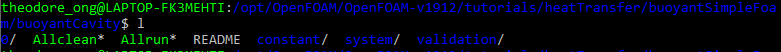
\includegraphics[width=6.27in,height=0.42in]{./media/image7.png}
	\end{Center}
\end{figure}


%%%%%%%%%%%%%%%%%%%% Figure/Image No: 6 Ends here %%%%%%%%%%%%%%%%%%%%

in 0 directory, we can remove everything except T U, p and P\_RGH, p\_rgh is pressure minus hydrostatic pressure\par



%%%%%%%%%%%%%%%%%%%% Figure/Image No: 7 starts here %%%%%%%%%%%%%%%%%%%%

\begin{figure}[H]
	\begin{Center}
		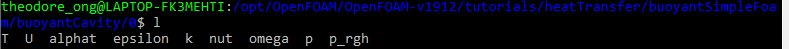
\includegraphics[width=6.27in,height=0.39in]{./media/image8.png}
	\end{Center}
\end{figure}


%%%%%%%%%%%%%%%%%%%% Figure/Image No: 7 Ends here %%%%%%%%%%%%%%%%%%%%

\par

Detailed BCs can do it later$ \ldots $ \par

In constant directory, we can use thermophysical properties from dowtherm A (from heat transfer)\par



%%%%%%%%%%%%%%%%%%%% Figure/Image No: 8 starts here %%%%%%%%%%%%%%%%%%%%

\begin{figure}[H]
	\begin{Center}
		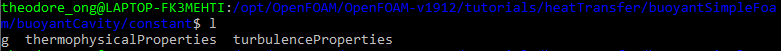
\includegraphics[width=6.27in,height=0.41in]{./media/image9.png}
	\end{Center}
\end{figure}


%%%%%%%%%%%%%%%%%%%% Figure/Image No: 8 Ends here %%%%%%%%%%%%%%%%%%%%

\par

Turbulence properties  laminar (not truly laminar but it just means I don’t use any model here)\par


\vspace{\baselineskip}
\subsubsection{BCs, fvSchemes, fvSolution}\par

For temp BCs, we have fixed temperature BCs and cyclic on all sides  relatively simple\par

For velocity BCs, we need to fix the mean flow and make it periodic\par

For Pressure BCs, we need to have a fixed pressure drop for fixed flow (one is calculated, one is fixed flux pressure drop)\par


\vspace{\baselineskip}
\textbf{fvSchemes}\par

\begin{itemize}
	\item As non dissipative as possible, central difference 2\textsuperscript{nd} order schemes (Gauss linear) would be best, fingers crossed on stability!\par

\end{itemize}
\textbf{fvSolution}\par
\begin{itemize}
	\item Not quite sure yet\par

	\item How do we iterate discretized equations\par

	\item What is P, pfinal\par
	\begin{itemize}
	\item \href{https://cfd.direct/openfoam/user-guide/v6-fvsolution/}{https://cfd.direct/openfoam/user-guide/v6-fvsolution/}\par

	\item Remember nCorrectors? Eg. Solving the pressure corrector in piso algorithm 4 times\par
\end{itemize}



\begin{itemize}
	\item First 3 times use the settings for p (usually error bigger here, so doesn’t converge as fast)\par

	\item Final time use settings for pfinal (smaller error here, so can be more stringent with tolerance)\par


\end{itemize}


\end{itemize}
GAMG or PCG? And what are preconditioners?\par

\begin{itemize}
	\item A good report here:\par

	\item \href{http://www.tfd.chalmers.se/~hani/kurser/OS_CFD_2008/TimBehrens/tibeh-report-fin.pdf}{http://www.tfd.chalmers.se/$ \sim $ hani/kurser/OS\_CFD\_2008/TimBehrens/tibeh-report-fin.pdf}\par

	\item We are solving systems of equations in matrices\par

	\item Eg  \( Ax=b \) \par

\begin{itemize}
	\item Preconditioner gives\par

\begin{itemize}
	\item  \( M^{-1}Ax=M^{-1}b \) \par

	\item This supposedly helps solve the matrix with less iterations or more stably\par


\end{itemize}
	\item Smoothers \par

\begin{itemize}
	\item Remember how preconditioners reduce no. of iterations?\par

	\item However as mesh grows $\#$  iterations also grows\par

	\item We can reduce this dependency with smoothers\par


\end{itemize}
	\item In general matrices are asymmetric\par

\begin{itemize}
	\item DILU is good for this (diagonal based incomplete LU decomposition)\par

\begin{itemize}
	\item Velocity equations are complex\par


\end{itemize}
	\item DIC class is good for symmetric matrices\par

\begin{itemize}
	\item Pressure equations are more symmetrical\par


\end{itemize}
\end{itemize}
\end{itemize}
\end{itemize}

Solvers \par

\begin{itemize}
	\item Now after preconditioning and smoothing we can think about solvers\par

	\item Detailed background here:\par

\begin{itemize}
	\item \href{https://www.youtube.com/watch?v=BApG0hasPf4&list=PLbMVogVj5nJS4AsBvnp9bCw0wAovDlXPl}{https://www.youtube.com/watch?v=BApG0hasPf4$\&$ list=PLbMVogVj5nJS4AsBvnp9bCw0wAovDlXPl}\par

	\item \href{https://www.foamacademy.com/wp-content/uploads/2018/03/OF2018matrix.pdf}{https://www.foamacademy.com/wp-content/uploads/2018/03/OF2018matrix.pdf}\par

	\item Krylov Subspace Methods \par

\begin{itemize}
	\item \href{https://www.youtube.com/watch?v=B_eSPrYuIuU}{https://www.youtube.com/watch?v=B\_eSPrYuIuU}\par


\end{itemize}
\end{itemize}
	\item GAMG \par

\begin{itemize}
	\item Multigrid solver  coarse mesh solve then map onto fine mesh (usually faster)\par


\end{itemize}
	\item Conjugate solvers (or some variation)\par

\begin{itemize}
	\item Exploits the conjugate vectors (not explaining here)\par

\begin{itemize}
	\item What are conjugate vectors?\par

\begin{itemize}
	\item Suppose we have a matrix A, and two vectors  \( \overrightarrow{v} \)  and  \( \overrightarrow{w} \) \par

	\item These are conjugate vectors of A if:  \( \overrightarrow{v}^{T}A\overrightarrow{w}=0 \) \par


\end{itemize}
\end{itemize}
\end{itemize}
	\item Gauss seidel (quite basic)\par
\end{itemize}

\textbf{Examples of fvSolution in OpenFOAM tutorials}

For dnsFoam boxTurb16, the following solvers are used:\par



%%%%%%%%%%%%%%%%%%%% Figure/Image No: 9 starts here %%%%%%%%%%%%%%%%%%%%

\begin{figure}[H]
	\begin{Center}
		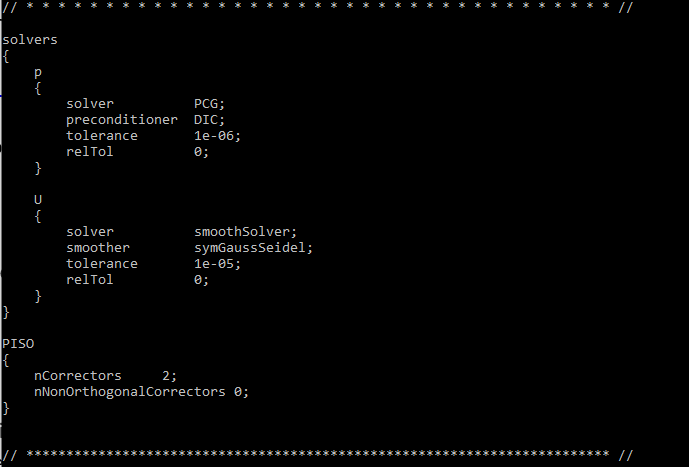
\includegraphics[width=6.27in,height=4.25in]{./media/image10.png}
	\end{Center}
\end{figure}


%%%%%%%%%%%%%%%%%%%% Figure/Image No: 9 Ends here %%%%%%%%%%%%%%%%%%%%

\par

In fireFoam, (quite challenging and non disspative)\par



%%%%%%%%%%%%%%%%%%%% Figure/Image No: 10 starts here %%%%%%%%%%%%%%%%%%%%

\begin{figure}[H]
	\begin{Center}
		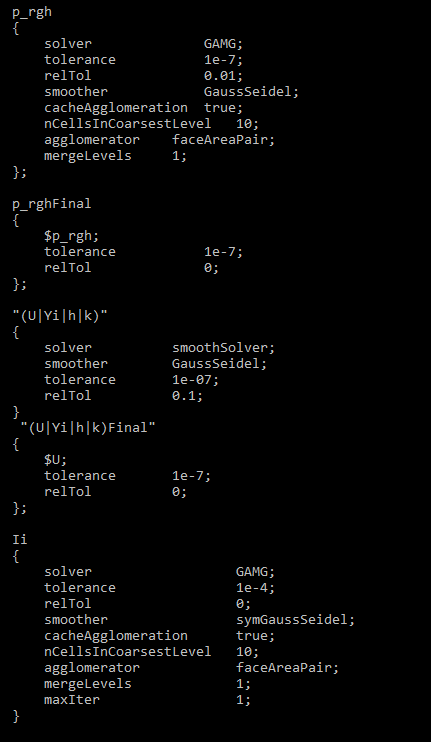
\includegraphics[width=4.49in,height=7.73in]{./media/image11.png}
	\end{Center}
\end{figure}


%%%%%%%%%%%%%%%%%%%% Figure/Image No: 10 Ends here %%%%%%%%%%%%%%%%%%%%

\par

Pressure, velocity, radiation all use gauss seidel or variants of such.\par

More on linear equation solvers\par

\href{https://www.openfoam.com/documentation/guides/latest/doc/guide-solvers.html}{https://www.openfoam.com/documentation/guides/latest/doc/guide-solvers.html$\#$ sec-solvers-intro}\par


\vspace{\baselineskip}
And how are fvSchemes setup?\par


\vspace{\baselineskip}
\par

I’ll try to make it as non dissipative as possible, eg. Linear or cubic interpolation, and use a stable solver, PCG for pressure and smooth solver for velocity, temperature.\par



\textbf{Periodic BCs}\par

How are cyclic BCs done in OpenFOAM?\par

\href{https://www.openfoam.com/documentation/guides/latest/doc/guide-bcs-coupled-cyclic.html}{https://www.openfoam.com/documentation/guides/latest/doc/guide-bcs-coupled-cyclic.html}\par

Consider the FlamePropagation with Obstacles case in PDRFoam under combustion in tutorials:\par

\par


\vspace{\baselineskip}
First we need to define which two patches are linked in blockMeshDict\par

\par

And in each BC, eg. In the changeDictionaryDict\par

\par

Define it as cyclic.\par

Another good place to look is LES channel395 tutorial\par

\href{https://www.openfoam.com/documentation/guides/latest/doc/guide-bcs-coupled-cyclic.html}{https://www.openfoam.com/documentation/guides/latest/doc/guide-bcs-coupled-cyclic.html}\par


\vspace{\baselineskip}
One question though, for pressure, we need fixed flux, though hydrostatic pressure will go through the roof because it’s $``$infinite length$"$ \par

How is this solved?\par

For one, I can fix it at 6m depth worth of hydrostatic pressure (or settle for atmospheric!)\par

I’ll have to experiment with this on a \uline{coarse mesh first} then go to fine mesh.\par

The other thing is this, \par

The total pressure field is all calculated, meaning to say that the hydrostatic pressure at the bottom is not added to the top, but rather the p\_rgh (pressure without hydrostatic component) is added and cyclic.\par

\href{https://www.openfoam.com/documentation/guides/latest/doc/guide-bcs-coupled-jump-fan.html}{https://www.openfoam.com/documentation/guides/latest/doc/guide-bcs-coupled-jump-fan.html}\par

fanPressure from TJunction will be most helpful\par

Ohh!!!\par

\textbf{\uline{No need to go through the trouble of fan and everything, this is easier:}}\par

\href{https://www.openfoam.com/documentation/guides/latest/doc/guide-fvoptions-sources-mean-velocity-force.html}{https://www.openfoam.com/documentation/guides/latest/doc/guide-fvoptions-sources-mean-velocity-force.html}\par

meanVelocityForce enables can fix the velocity\par
\begin{itemize}
	\item We want mean velocity to be: 0.307959467 m/s\par

\end{itemize}


\vspace{\baselineskip}
When I run the thing, im shown that cyclic conditions \uline{cannot} use calculated.\par

\uline{Data collection examples in OpenFOAM Tutorials}\par

Where can I go to obtain graphical data generation templates?\par

Firstly postChannel from channel395 is an interesting way to start data collection$ \ldots $ \par
\begin{itemize}
	\item But I’ll probably need to store obscene amounts of data on the computer, I need graphs created at certain timesteps. In fact, every 0.4s I want a graphical chart of data.\par

	\item Plus I want heat transfer c\par
\end{itemize}


One start point is here:\par

\href{https://cfd.direct/openfoam/user-guide/v6-post-processing-cli/}{https://cfd.direct/openfoam/user-guide/v6-post-processing-cli/$\#$ x31-2450006.2.1.9}\par

singleGraph option is good, we can look in laminar planarPoiseuille\par

\par

Also my hotSphere in oil case$ \ldots $  I run functionObjects during runtime\par

I wish to purgewrite the data off, but preserve maybe 6 timesteps tops, thankfully data is listen in postprocessing on the fly.\par

Looks like that’s it$ \ldots $  I’ll need to try it out.\par


\vspace{\baselineskip}
\textbf{functionObjects OpenFoam Examples}\par

Surface field values (see hot sphere in oil case)\par

\begin{itemize}
	\item Wall Shear stresses\par

	\item Average Heat transfer Coefficients \par


\end{itemize}
Sets (see buoyantCavity Case)\par

\href{https://www.openfoam.com/documentation/guides/latest/doc/guide-fos-sampling-sets.html}{https://www.openfoam.com/documentation/guides/latest/doc/guide-fos-sampling-sets.html}\par

\href{https://develop.openfoam.com/Development/openfoam/-/blob/master/tutorials/heatTransfer/buoyantSimpleFoam/buoyantCavity/system/sample}{https://develop.openfoam.com/Development/openfoam/-/blob/master/tutorials/heatTransfer/buoyantSimpleFoam/buoyantCavity/system/sample}\par


\vspace{\baselineskip}
After doing a RANS run coarse mesh (10 by 10 by 10), realise it is more efficient to run it to convergence and map this temperature and velocity field to dns.\par

So I run RANS for 100s simulated time, map fields and run quasiDNS 40s simulated time\par

Can we set up a run file for this?\par

From mapfields cavity, case, we get a rather interesting way$ \ldots $ \par

\par

\section{First Run of QuasiDNS}\par

With this cell level, of refinement, the computer froze trying to run blockMesh.\par

And like 5 mins later, the blockMesh still isn’t complete. This doesn’t bode well for actual DNS.\par


\vspace{\baselineskip}
 \[ kolmogorov scale  \sim   \Delta x^{+}=1.83 \] \par

For OpenFOAM, (Komen et al., 2014), wall parallel directions: \(   \Delta x^{+}=9,~  \Delta z^{+}=4.5 \)   \(  \Delta y^{+}=0.8-4.5 \) , \par

Meaning to say, in y direction, $\frac{1}{2}$ Kolmogorov scale is sufficient to resolve near wall, 2x Kolmogorov scale far from wall.\par


\vspace{\baselineskip}

\vspace{\baselineskip}
Split domain in half. Largest cell is 4x of smallest cell.\par

\textbf{Streamwise direction}\par

Cell size $ \sim $  4x Kolmogorov scale (\cite{Komen2014})\par

 \[ \frac{l}{ \eta }=\frac{1\ast8}{0.002350377\ast4} \approx 851 cells \] \par

\textbf{Spanwise direction}\par

Cell size $ \sim $  2x Kolmogorov scale (\cite{Komen2014})\par

 \[ \frac{l}{ \eta }=\frac{1\ast3}{0.002350377\ast2} \approx 639 cells \] \par

Total no. of cells:\par

 \[ 2.32E+08 \approx 232 million \] \par

This is 426 in y direction, 852 streamwise, 639 spanwise.\par

That’s a LOT, note: LES simulations can be on order of  \( \text{0.3 million} \)  cells.\par

\section{2nd Run of QuasiDNS - get blockMesh to generate less cells}

Need to reduce cells to about 1-2 million. Meaning 10x less cells in x and y direction. (z I cannot compromise too much)\par

Means streamwise, we get $ \sim $  cell size of 40x Kolmogorov scale streamwise and 20x Kolmogorov scale in spanwise, and then we get 1x-4x Kolmogorov in wall normal direction.\par

Use kOmegaSST-IDDES since that has proven to be useful and it’s convenient (kOmegaSST fields are set well)\par

Note that about 80s later, the average heat trf coefficient settles down.\par

Good rule of thumb: 1 million cells  1 GB ram required for mesh\par


\vspace{\baselineskip}
Alternative 2 would be to lessen the domain spanwise and streamwise by 10x. This preserves mesh grading but may neglect large turbulence structure formation. (I’m suppressing large eddy formation)\par

Hard limit on computer is about 2-4 million cells.\par


\vspace{\baselineskip}

\subsection{Quantify ${y}^{+}$ so that i can coarsen the mesh}
Anyhow, wall shear stress is  \(  \tau_{wall} \approx 4.14\ast10^{-1} \)  according to RANS calcs (Re = 3200)\par

Friction velocity is:\par

 \[ u_{ \tau}=\sqrt[]{\frac{ \tau_{wall}}{ \rho }}=\sqrt[]{\frac{0.414}{1019}}=0.020156405\frac{m}{s} \] \par

Kolmogorov scale is about  \( 7\ast10^{-6}m \) \par

 \[ \frac{ \eta }{l} \sim \frac{1}{3200^{0.75}}=0.002350377 \] \par

Based on 1.5cm length,\par

 \[  \eta =3.53\ast10^{-5} \approx 35 microns \] \par

This corresponds to:\par

 \[ y^{+}=\frac{y \left[ m \right] u_{ \tau} \left[ \frac{m}{s} \right] }{ \nu  \left[ \frac{m^{2}}{s} \right] }=\frac{3.53\ast10^{-5}\ast0.02}{1.44\ast10^{-6}}=4.88E-01 \approx 0.5  \] \par

1 kolmogorov scale is approx. 0.5  \( y^{+} \) !\par

My smallest mesh size is about 0.25  \( y^{+} \)  (1/2 kolmogorov scale)\par

At the right side,\par

 \[ u_{ \tau}=\sqrt[]{\frac{ \tau_{wall}}{ \rho }}=\sqrt[]{\frac{0.464}{1019}}=0.0214\frac{m}{s} \] \par

Doesn’t actually change the  \( y^{+} \)  too much!\par

 \[ y^{+}=\frac{y \left[ m \right] u_{ \tau} \left[ \frac{m}{s} \right] }{ \nu  \left[ \frac{m^{2}}{s} \right] }=\frac{3.53\ast10^{-5}\ast0.0214}{1.44\ast10^{-6}}=5.23E-01 \approx 0.523 \] \par

1 kolmogorov scale is enough to be the smallest which means I can halve my cell requirements in y direction.\par


\vspace{\baselineskip}
This is 213 in y direction, 852 streamwise, 639 spanwise.\par

Likewise, in streamwise direction, I’m having 4 kolmogorov scales\par

 \[  \Delta x^{+} \approx 2.1 \] \par

I can decrease cell count by 4x and still be within guidelines\par

 \[  \Delta x^{+} \approx 8.4  \left( streamwise \right)  \] \par


\vspace{\baselineskip}
 This is 213 in y direction, 213 streamwise, 639 spanwise.\par

Finally, spanwise, im also too strict, being 3 kolmogorov scales,\par

 \[  \Delta z^{+} \approx 1.5 \] \par

I can decrease it 3x\par

 \[  \Delta z^{+} \approx 4.5  \left( spanwise \right)  \] \par


\vspace{\baselineskip}
This is 213 in y direction, 213 streamwise, 213 spanwise.\par

This makes for about 9.66 million cells, way more doable (but I’m really pushing it)\par

\textbf{Running blockMesh for this, about 95$\%$  of free ram was used, computer went hanging for 15 mins}\par

\section{The $3^{rd}$ run, reduce no. of cells due to RAM limit of 8GB}
Should push it down as far as possible, try Re=2350 mixed convection.\par

 \[ 213\ast\frac{2350}{3200}=157 \] \par

 \[ 157^{3}=3827300 cells \approx 3.9 million cells \] \par

That is 3.9 million cells. That’s about the best we can manage$ \ldots $ \par

\textbf{For LES type:}\par

157$\ast$ 40$\ast$ 40 \par

 Or 158/2 =79 cells\par

\textbf{For RANS type}\par

157$\ast$ 4$\ast$ 4 \par

Velocity is now\par

 \[ 0.307959467\ast\frac{2350}{3200} \approx 0.22618\frac{m}{s} \] \par

 Wall shear stress is now (in RANS mode)  estimated\par

 \[ u_{ \tau}=\sqrt[]{\frac{ \tau_{wall}}{ \rho }}=\sqrt[]{\frac{0.27}{1019}}=0.0162777\frac{m}{s} \] \par

New Kolmogorov scale is:\par

 \[ \frac{ \eta }{l} \sim \frac{1}{2350^{0.75}}=0.002962 \] \par

Note that this is still smaller than the Kolmogorov scale of natural convection:\par

 \[ \frac{ \eta _{k}}{H}= \left( \frac{Pr^{2}}{ \left( Nu-1 \right) Ra} \right) ^{\frac{1}{4}}=\frac{ \eta _{B}}{H}\ast\sqrt[]{Pr}=0.013357476\ast\sqrt[]{19}=0.0582 \] \par

So we’ll use the forced convection kolmogrov scale as reference.\par

 \[  \eta =0.015m\ast0.002962=4.444\ast10^{-5} \approx 44 \mu m \] \par

In terms of  \( y^{+} \)  units, Kolmogorov scale is:\par

 \[ y^{+}=\frac{y \left[ m \right] u_{ \tau} \left[ \frac{m}{s} \right] }{ \nu  \left[ \frac{m^{2}}{s} \right] }=\frac{4.44\ast10^{-5}\ast0.0162777}{1.44\ast10^{-6}}=5.02368E-01 \approx 0.503 \] \par

Looks good! Kolmogorov scale =1/2  \( y^{+} \)  ish\par

Can live with this  in fact wall shear stress decreases as the simulation stablilises.\par

 \[ Re_{ \tau}=\frac{0.0162777\ast0.015}{1.44\ast10^{-6}} \approx 169 \] \par

(low level turbulence)\par

Note that I use a Prt of 0.85 throughout in all these. Though for RANS, probably used Prt =0.85 near wall, 1 in bulk fluid.\par


\vspace{\baselineskip}
Okay if you copy and paste the files over, run mapFields for t=100s.\par

Source file shows coarse mesh\par

Target file must show fine mesh (but now it doesn’t do that yet.)\par

So I need to run RANS in the other folder and then map the fields over!\par

For IDDES,\par

Estimated  \( u_{ \tau} \) \par

Is at\par

 \[ u_{ \tau}=\sqrt[]{\frac{ \tau_{wall}}{ \rho }}=\sqrt[]{\frac{0.29}{1019}}=0.0169\frac{m}{s} \] \par

 \[ y^{+}=\frac{y \left[ m \right] u_{ \tau} \left[ \frac{m}{s} \right] }{ \nu  \left[ \frac{m^{2}}{s} \right] }=\frac{4.44\ast10^{-5}\ast0.0169\frac{m}{s}}{1.44\ast10^{-6}}=5.201E-01 \approx 0.52 \] \par

 \[ \frac{ \eta }{l} \sim \frac{1}{ \left( 2350^{0.75} \right) } \] \par

 \[ \frac{l}{ \eta } \sim 337.52 \] \par

Divide by two\par

And we need $ \sim $ 169 cells in each direction.\par

 \[ 169^{3} \approx 4.8268 million cells \] \par


\vspace{\baselineskip}
Still acceptable\par

In streamwise direction we have about 16 nodes\par

Distance is:\par

 \[  \Delta x_{IDDESSize}^{+}=\frac{\frac{0.12}{16}m\ast0.0169\frac{m}{s}}{1.44\ast10^{-6}}=87.86 \] \par

This is not quite LES size mesh$ \ldots $  not LES, need it about  \(  \Delta x^{+} \approx 40 \) ,\par

Good for mesh refinement study anyhow$ \ldots $ \par

 \[ u_{ \tau}=\sqrt[]{\frac{ \tau_{wall}}{ \rho }}=\sqrt[]{\frac{0.31}{1019}}=0.0175\frac{m}{s} \] \par

 \[  \Delta y^{+} \left( \text{158 cells mesh} \right) =\frac{\frac{0.015m}{158}\ast0.0175\frac{m}{s}}{1.44\ast10^{-6}}=1.154 \] \par

Smallest cell size:\par

 \[  \Delta y_{smallest}^{+}=\frac{1.154}{2}=0.5768 \] \par

In x direction (streamwise)\par


\vspace{\baselineskip}
 \[  \Delta z_{159-cell}^{+}=\frac{\frac{0.12}{159}m\ast0.0175\frac{m}{s}}{1.44\ast10^{-6}}=9.171  \left( streamwise \right)  \] \par

Recommended size (streamwise)  \(  \Delta z_{stream}^{+}=9 \) \par

Spanwise,\par

 \[  \Delta x_{159-cell}^{+}=\frac{\frac{0.045}{159}m\ast0.0175\frac{m}{s}}{1.44\ast10^{-6}}=3.057  \left( spanwise \right)  \] \par


\vspace{\baselineskip}
So basically, increase mesh refinement 3x in x and z direction to get proper LES length scale\par

Reduce by 10x ish (to 157 cells) to get DNS length scale\par

Oops I used 157 mesh not 159\par

In x direction (streamwise)\par


\vspace{\baselineskip}
 \[  \Delta z_{159-cell}^{+}=\frac{\frac{0.12}{157}m\ast0.0175\frac{m}{s}}{1.44\ast10^{-6}}=9.288  \left( streamwise \right)  \] \par

Recommended size (streamwise)  \(  \Delta z_{stream}^{+}=9 \) \par

Spanwise,\par

 \[  \Delta x_{159-cell}^{+}=\frac{\frac{0.045}{159}m\ast0.0175\frac{m}{s}}{1.44\ast10^{-6}}=3.096  \left( spanwise \right)  \] \par


\vspace{\baselineskip}

\vspace{\baselineskip}
Anyhow testing DNS mesh size for blockMesh$ \ldots $ \par

\par

Really Pushes the computer to the limit. That’s about all it can manage.\par

Huge Ram requirements. But it’s a DNS mesh$ \ldots $  what do you expect :) \par

Note file size for the polymesh also!!\par

(ls -lh command)\par

\par

380 Mb just for one polymesh file.\par

Takes about 1-3 minutes to blockMesh and mapFields\par

Likely I’ll need to make purgewrite 1 to delete all other files besides last written timestep. \par

Quite an insane memory requirement.\par

Running pimpleFoam on this mesh froze my computer$ \ldots $ \par


\vspace{\baselineskip}
So I would like to take advantage of mesh in x direction, decrease it to 125 cells, and increase z cells to 162\par

Total mesh number is:\par

 \[ \#cells=125\ast158\ast162=3199500 cells \approx 3.2 million \] \par

Looks like my hardware can only take 3 million is cells.\par

Secondly we have instability growth here$ \ldots $ \par

\par

System is unstable here$ \ldots $ \par

Let’s solve one thing at a time.\par
\section{The $4^{th}$ run, and several debugs}

\subsection{First let's find the upper limit of blockMesh}$ \ldots $ \par

\begin{itemize}
	\item Max memory $ \sim $  3.2 GB used, and it’s much faster, felt like 1/3 of time\par

	\item Looks good! Now let’s see buoyantPimpleFoam, did it freeze the computer?\par

\par

Looks okay, just bearable.\par

Yup so 3.2 million cells is the upper limit. NO MORE THAN THIS.\par

\end{itemize}

Takes about 1 minute to compute one time step.\par

\subsection{Let's see the upper limit on time}
So how long will it take if this is stable?\par

 \[ total time=100s \left( sim \right) \ast\frac{\text{1 min} \left( real \right) }{2e-4s  \left( sim \right) }=500,000min=8334 hrs=347 days  \left( 1 year \right)  \] \par


\vspace{\baselineskip}
With this speed, 40s  140 days (5 months) 1 entire semester!\par

What about write time?\par

0.4s\par

 \[ total time=0.4s \left( sim \right) \ast\frac{\text{1 min} \left( real \right) }{2e-4s  \left( sim \right) }=2000 min=33.33hrs \] \par

I’d like it once per half hour..\par

Perhaps 0.004s is better, that should be the write time.\par

\subsection{Coarse Mesh IDDES and RANS buoyantPimpleFoam can resolve, but not fine mesh DNS with buoyantPimpleFoam}

\uline{Now that calculation is long but manageable, I realise that another issue crops up when I do fine mesh  buoyantPimpleFoam doesn’t really resolve fine mesh instabilities well, only coarse mesh LES works and RANS too, any smaller and the solver becomes unstable}\par

Suppose the time issue is ok, then how about the instability issue?\par

\subsection{Do LES fine mesh  introduce some viscosity to control oscillation, may help control turbulence,}\par

Given of course that LES is meant to tend to DNS if the mesh is ultra small. (Kolmogorov scale)\par

(characteristic lengthscale tends to 0 anyhow) so this should be ok\par

Second is to change controlDict to use constant timestep?\par

Suspicion: starting timestep too small.\par


\vspace{\baselineskip}
Anyhow Co seems to drop below 1 (oscillating)\par

Okay instabilities growing$ \ldots $ \par


\subsection{Try introducing pimple Loop nOutercorrectors to stabilise the system}

\href{https://www.researchgate.net/post/Why_do_calculations_blow_up_when_using_finer_grids_k-omega_SST}{https://www.researchgate.net/post/Why\_do\_calculations\_blow\_up\_when\_using\_finer\_grids\_k-omega\_SST}\par

2 ways to resolve numerical stability in fine mesh according to the post:\par

Increase nOuterCorrectors in Pimple loop to 3\par

\begin{itemize}
	\item Linear upwind scheme used\par
\begin{itemize}
	\item Increase no. of cells\par
	\item Upwind scheme more dispersive, so need to increase no. of cells for DNS

\end{itemize}

\end{itemize}

I’ll try the pimple loop first.\par

This was kOmegaSSTIDDES with DNS sized mesh (based on Kolmogorov scale)\par

Okay this didn’t work$ \ldots $ \par

Probably the viscosity was too small to even make a difference due to small mesh size\par

\subsection{I’m going to try eliminating solvers as a problem, probably Gauss Siedel solver is more stable than PCBiCG Solver}\par

I’m going to try smooth solver Gauss seidel in fvSOlutions as per dnsFoam boxTurb16\par

Solver doesn’t work! \par

\subsection{Now if the timestep is too small, the solver becomes unstable for some reason, so I don’t adjust timestep to be smaller, but fix it instead}\par

Next I can try fixing the timestep\par

Use runtime instead\par

I’ll write data every 20 min\par

\href{https://cfd.direct/openfoam/user-guide/v6-controldict/}{https://cfd.direct/openfoam/user-guide/v6-controldict/}\par


\vspace{\baselineskip}
With parallel processing, I get 1.5 min per timestep..\par
\begin{itemize}
	\item But the memory usage is a lot less now, 3.4 GB as compared to 4ish GB
\end{itemize}\par

Anyhow instability developed, pimpleFoam not able to run.\par

\subsection{Trying out GAMG matrix solver to see if fvSolution is the problem}\par

I’m going to try GAMG for U to see if this works to stabilise things$ \ldots $ \par

Doesn’t seem to, \par

Let me use a bigger timestep instead!\par

 \[ Co=\frac{v \Delta t}{l_{cell}}=\frac{0.22618\ast \Delta t}{\frac{0.074074}{100}}=3.053\ast10^{2} \Delta t \] \par

For Co=0.5\par

 \[  \Delta t=\frac{0.5}{3.053\ast10^{2}}=0.001677s \approx 0.0015s \] \par


\subsubsection{i suspect having a varying timestep that was adjusting the timestep too small was an issue, and tried eliminating that}
Maybe it’s too small a timestep causing the error!\par

Changing timestep to 1.5e-3\par

Going back to symmetric Gauss seidel smoother smooth solver  this was faster and yielded the same results\par

So regardless of solver it looks the same!\par

And smooth solver gauss seidel solver takes less memory than GAMG as well! (3.4 GB vs 4 GB when running buoyantPimpleFoam in serial)\par

It turns out unstable and the max iterations for k and omega are reached.\par

\begin{itemize}

	\item I’ll remove k and omega from calculation\par

\end{itemize}

\vspace{\baselineskip}
\subsection{k and omega reached max iterations in last calculation, i turned off the turbulence model to see if that could help with stabiltiy}
Okay this still results in instability.\par

Courant number blows up to 18.\par

\subsection{Perhaps my discretisation schemes in fvSchemes is the problem, though I don’t really want to mess with it since it gives me less accuracy}\par
However, in less resolved meshes, it seems to work  I posit that dissipation adds to stability. Therefore, I’ll try to use dissipation schemes (upwind) for conduction.\par

Let me try Gauss Upwind for div(phi,h) these are convective terms.\par

Ok that doesn’t work$ \ldots $ \par
\subsection{I don't know what to do, but i want to look online to see if same problems are encountered and if there are solutions}

 Are there any people doing dns that have done it online?\par

\href{https://bugs.openfoam.org/view.php?id=1894}{https://bugs.openfoam.org/view.php?id=1894}\par

This is one,\par

This is his code:\par

ddtSchemes\par

$ \{ $ \par

\ \ \ \ default\ \ \ \ \ \ \   CrankNicolson 0.9;//backward;//CrankNicolson 1.0;//\par

$ \} $ \par


\vspace{\baselineskip}
gradSchemes\par

$ \{ $ \par

\ \ \ \ default\ \ \ \ \ \ \   Gauss linear;\par

$ \} $ \par


\vspace{\baselineskip}
divSchemes\par

$ \{ $ \par

\ \ \ \ default\ \ \ \ \ \ \   none;\par

\ \ \ \ div(phi,U)\ \ \ \   Gauss linear;//midPoint;//\par

\ \ \ \ div(phi,h)\ \ \ \   Gauss QUICK phi;//\par

\ \ \ \ div(phi,e)\ \ \ \   Gauss linear;\par

\ \ \ \ div(phi,K)\ \ \ \   Gauss linear;\par

\ \ \  div(phi,epsilon) Gauss linear;\par

\ \ \ \ div(phi,R)\ \ \ \   Gauss linear;\par

\ \ \ \ div(phi,Ekp)\ \   Gauss linear;\par

\ \ \ \ div(R)\ \ \ \ \ \ \ \   Gauss linear;\par

\ \ \  div((muEff$\ast$ dev2(T(grad(U))))) Gauss linear;// corrected;\par

$ \} $ \par


\vspace{\baselineskip}
\href{https://www.openfoam.com/documentation/user-guide/fvSchemes.php}{https://www.openfoam.com/documentation/user-guide/fvSchemes.php}\par

according to this, gauss quick phi is one way to do it$ \ldots $ \par

\uline{next I want to eliminate a bad initial condition where the initial condition is so far from actual solution that it causes instability, I’d want to have an initial condition with some semblance of turbulence to allow DNS to catch up so to speak}\par

Another note: when I reduce mesh size, for the first few seconds, wall shear stress drops dramatically.\par

\begin{itemize}
	\item 0.261 initially for IDDES case 1: mesh size  \(  \Delta z^{+} \left( streamwise \right) = \) 89\par

	\item Then for first timesteps, the average wall shear stress was 1.733e-1 (0.17)\par

	\item Only went back to 0.245 a few seconds later\par

	\item This lack of wall shear stress probably due to modelled stress depletion (suddenly  \(  \nu _{t} \)  disappears and now turbulence is expected to be resolved) may be a factor in causing such a thing.\par
\end{itemize}



Thus the initial velocity profiles for less resolved cases may cause certain instabilities esp near wall?\par

Not really sure$ \ldots $ \par
\subsection{Perhaps mapping fields from a coarse solution caused it to blow up?}
But if I DNS from scratch will this issue re-alppear?\par

Anyway IDDES finer mesh solver blew up as well\par

\subsection{maybe dpdt term in buoyantPimpleFoam causes problems}
\uline{So trying the above, i thought something else must be the issue, I wondered if other people were facing the same issue as i}\par
\href{https://www.cfd-online.com/Forums/openfoam-solving/220924-highly-unstable-buoyantpimplefoam-simulation.html}{https://www.cfd-online.com/Forums/openfoam-solving/220924-highly-unstable-buoyantpimplefoam-simulation.html}\par

One former here suggested dpdt off$ \ldots $ \par

We can try that.\par

Courant number still grows$ \ldots $ \par


\vspace{\baselineskip}
Anyhow to run in parallel, use:\par

Mpirun -np 4 buoyantPimpleFoam -parallel $\&$ \par

\subsection{Looks like many people online face the same issue!}
\href{https://www.cfd-online.com/Forums/openfoam-solving/220924-highly-unstable-buoyantpimplefoam-simulation.html}{https://www.cfd-online.com/Forums/openfoam-solving/220924-highly-unstable-buoyantpimplefoam-simulation.html}\par

Pimplefoam unstable at small courant numbers, not the first time!\par

\href{https://www.cfd-online.com/Forums/openfoam-solving/172144-pimplefoam-rhopimplefoam-unstable-small-courant-numbers-time-steps.html}{https://www.cfd-online.com/Forums/openfoam-solving/172144-pimplefoam-rhopimplefoam-unstable-small-courant-numbers-time-steps.html}\par


\vspace{\baselineskip}
\textcolor[HTML]{4472C4}{$``$Folks - I have not reviewed your cases in detail, but let me offer the following observation to see if it helps.}\par


\vspace{\baselineskip}
\textcolor[HTML]{4472C4}{Reducing the time step significantly will reduce your temporal differencing errors ... if this is first order temporal differencing then you are removing some of the numerical stabilising (damping) that is present in your high Co runs. That is probably why your low Co runs are much more lively.}\par


\vspace{\baselineskip}
\textcolor[HTML]{4472C4}{You see the same effect when refining mesh spacing - what runs nice and stably with a coarse mesh can go haywire as you refine the mesh and remove the numerical diffusion that is stabilising the solution.$"$  – Tobermory}\par

\subsection{Thermal Diffusion timescales not resolved, thus instability? let's test}

\uline{One other possibility is that my time scales are not small enough to resolve heat transfer, usually this case of instability comes with heat transfer because we have negative temperatures}\par


I’m going to try the crank Nicolson time scheme now, cos that seems to be the most logical (two other folks with working simulations use this$ \ldots $ ) \par

Still blew up:\par

One more timescale to consider:\par

\href{https://en.wikipedia.org/wiki/Von_Neumann_stability_analysis}{https://en.wikipedia.org/wiki/Von\_Neumann\_stability\_analysis}\par

 \[ \frac{ \alpha  \Delta t}{ \Delta x^{2}} \leq 0.5 \] \par

Larger alpha is more conservative\par

 \[ Pr=\frac{ \nu }{ \alpha } \] \par

 \[  \alpha =\frac{ \nu }{Pr}=\frac{1.443e-6}{15}=9.62e-8  \] \par

 \[ \frac{ \alpha  \Delta t}{ \Delta x^{2}} \leq 0.5 \] \par

Kolmogorov lengthscale  \(  \eta =\frac{0.015m}{157}= \) \par

 \[ 9.62e-8 \left( \frac{m^{2}}{s} \right) \ast\frac{2e-4s}{95 \mu m^{2}}=0.0021077 \] \par

So tis criteria is met. Nothing to do with this.\par

\part{Putting DNS on hold, let's try LES with a proper LES mesh first}

\uline{Okay, so DNS isn’t working, I’ll try something simpler first: IDDES with LES type mesh}\par

\section{IDDES Case 2: Proper LES mesh, Run 1}
$\Delta x ^{+}\approx 40$

I’m also trying crank Nicolson for IDDES case 2, with LES type mesh. Initial results seem stable.\par

But after 0.15s simulation time, the simulation blows up.\par
\begin{itemize}
	\item Interesting thing, the courant number has growing oscillations about Co=0.5, indicative of some oscillation.\par
\end{itemize}

\subsubsection{More Reads online show that buoyantPimpleFoam Instability is a common issue}

Next interesting thing, when I search buoyantPimpleFoam velocity oscillations, i see a few people’s master’s thesis and they experience the same problem.\par


\begin{itemize}
	\item In fact they could not finish their thesis when they tried various things, fvSchemes, relaxation factors, BCs etc.\par

	\item Common problem, im not alone\par

	\item Eg. \href{https://fenix.tecnico.ulisoba.pt/downloadFile/1689244997257061/tese.pdf}{https://fenix.tecnico.ulisoba.pt/downloadFile/1689244997257061/tese.pdf}\par

	\item www5.in.tum.de/pub/Cheung2016\_Thesis.pdf\par

	\item Some ignore buoyancy altogether\par
\end{itemize}

\subsubsection{Batchelor Scales apply to Forced convection! not just natural convection}
As I read some things (Steven Van Haren thesis)\par

I realise batchelor scales also apply to Forced convection!\par

\begin{itemize}
	\item  \(  \eta _{B}=\frac{ \eta }{\sqrt[]{Pr}}~ \left( \text{dowtherm type }Pr>1 \right) \text{, or } \eta _{B}=\frac{ \eta }{Pr^{\frac{3}{4}}} \left( for Pr \leq 1 \right)  \)  (Haren, 2011)\par

\begin{itemize}
	\item G.K. Batchelor. Small-scale variation of convected quantities like temperature in turbulent fluid. Fluid Mech, 5:113–133, 1958.\par

	\item P.A. Davidson. Turbulence. Oxford University Press, 2004\par


\end{itemize}
	\item \href{https://repository.tudelft.nl/islandora/object/uuid:67186c81-cac5-41b6-a21f-8e3670cafead}{https://repository.tudelft.nl/islandora/object/uuid:67186c81-cac5-41b6-a21f-8e3670cafead} \par
\end{itemize}

 Oh bother..\par

This means that I need way finer, way way finer mesh.\par
\subsubsection{Do i need a finer mesh for Batchelor scales? and how much finer?}
But some mixed convection DNS use the mesh stated above$ \ldots $ \par

Nevertheless, the DNS done is usually for air, with Pr $\approx$ 0.71. Dowtherm has high Pr, may still need finer mesh to resolve Batchelor scales.

\section{IDDES Run 2, suspect that system is unable to cope going from start state to steady state, change in temperature too steep}
\uline{Is initial condition still the problem? Ie is initial condition so far from actual solution that the solver blows up?}\par

One way to circumvent is using a slightly bigger mesh, and use the well conditioned flow field to go down to DNS.\par

This is 36 x 158 x 36\par

This ensures max  \(  \Delta x^{+} \approx 39.11 \) \par

Still blows up.\par


\section{IDDES Run 3, suspect Batchelor scales are not properly resolved in IDDES, thus refine mesh and lower time to account for that}
\uline{Batchelor scale hypothesis}\par

I posit that when I reduce the size of the mesh,  \(  \nu _{sgs} \)  drops dramatically (because of smaller mesh size) so that resolved turbulence can make up for the loss of modelled viscosity.\par

However, on the heat transfer end,  \(  \alpha _{sgs} \)  also drops due to  \(  \nu _{sgs} \)  decreasing. But the Batchelor scales may be smaller than Kolmogorov scales. I calculated batchelor scales for natural convection, thinking it doesn’t apply to forced convection.\par


\vspace{\baselineskip}
But batchelor scales also apply to forced convection! It is just that when air is used, the Reynold’s analogy can hold well as  \( Pr \rightarrow 1 \) .\par

 \(  \eta _{B}=\frac{ \eta }{\sqrt[]{Pr}}  \left( dowtherm type Pr>1 \right) , or  \eta _{B}=\frac{ \eta }{Pr^{\frac{3}{4}}} \)  (\cite{Haren2011}) \par

\vspace{\baselineskip}
Therefore, when I decrease mesh size and  \(  \nu _{sgs} \) , the resolved turbulence increase   \( \overline{u^{'}v^{'}} \)  can make up for the loss in  \(  \alpha _{sgs} \)  and hopefully resolved turbulent heat flux   \( \overline{u'T'} \)  can also make up for the loss in  \(  \alpha _{sgs} \) .\par

However, when we have high Prandtl number fluids such as water and dowtherm A, forced convection batchelor scales become important. Most of the instability issues arise from water which has  \( Pr \)  of 5-7.\par

 \[  \eta _{B}=\frac{ \eta }{\sqrt[]{7}}=0.377 \eta   \] \par

Thus reducing mesh size to Kolmogorov scale in IDDES will resolve most fluid motion, but not resolve the Batchelor scales.\par

Van Haren’s thesis uses  \( Pr=1 \) . This allows for the reynold’s analogy to be used.\par

However, for  \( Pr=7 \) , Batchelor scales will come into play. Does it mean we refine in 3D? No. He writes that increasing fidelity in wall normal direction is sufficient.\par

These two papers were cited:\par

Y. Na and T.J. Hanratty. Limiting behavior of turbulent scalar transport close to a wall. Int. Journal of Heat and Mass transfer, 43:1749–1758, 2000.\par

R Bergant. Turbulent Heat Transfer near the Flat Wall for High Prandtl Numbers. PhD thesis, University of Ljubljana, Faculty of Mathematics and Physics, 2005.\par

So there are two ways of approaching this:\par

\begin{enumerate}
	\item I do the IDDES simulation with air as a fluid, but I’ll have to change grashof numbers etc\par

	\item I refine the y normal direction according to batchelor scale, not Kolmogorov and work from there.
\end{enumerate}\par
\subsubsection{Smallest scales of Batchelor scale and its impact on mesh size}
For this I’ll need a mesh of:\par

 \[ \frac{ \eta _{B}}{ \eta }=\frac{1}{\sqrt[]{Pr}} \] \par

For us, highest Pr number is $ \sim $ 28-30\par

 \[ \frac{ \eta _{B}}{ \eta }=\frac{1}{\sqrt[]{30}}=0.182 \] \par

In other words\par

 \[ \frac{ \eta }{ \eta _{B}} \approx 5.5 \] \par

So I’ll need to increase mesh refinement in y normal direction 5 times to capture Batchelor scale.\par

So mesh refinement is up to 395.\par



%%%%%%%%%%%%%%%%%%%% Figure/Image No: 11 starts here %%%%%%%%%%%%%%%%%%%%

\begin{figure}[H]
	\begin{Center}
		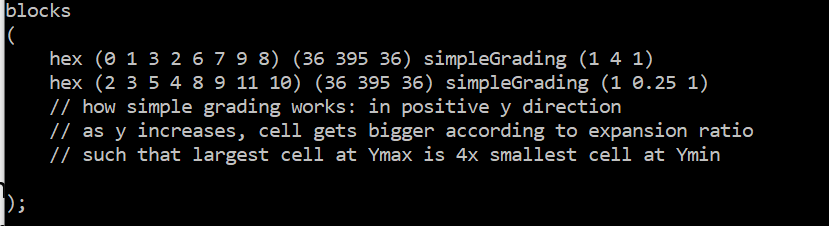
\includegraphics[width=6.27in,height=1.71in]{./media/image22.png}
	\end{Center}
\end{figure}


%%%%%%%%%%%%%%%%%%%% Figure/Image No: 11 Ends here %%%%%%%%%%%%%%%%%%%%

\par

This should capture properly all batchelor scales.\par
\paragraph{I probably need a better PC} \par 


However, doing this will ensure that I cannot even do DNS on this computer unless I reduce the size of the domain by 5 times also.\par


\begin{itemize}
	\item This will be interesting to test if available, a smaller domain DNS for air, compare to Kim and Menon for heat flux, wall normal profile. Nevertheless, it WILL take long.\par

	\item 3.2 million cells x5  \(  \approx 16 million cells \) \par

	\item I will need a 32 GB ram machine to calculate this comfortably\par
\end{itemize}


\paragraph{Lowering Timescales to resolve Batchelor Scales}
Likewise I need to make sure the speed of the turbulent heat flux does not exceed what is required similar to how Co is being done$ \ldots $ \par

The heuristic is that if the batchelor scale is 5.5x lower than the Kolmogorov scale, the batchelor timescale should be 5.5x lower than the Kolmogorov timescale.\par

Ie the courant number should be  \( =\frac{0.5}{5.5}=0.09 \) \par

So I’ll set that in the controlDict.\par

Now it’s running.\par

One thing though, this IDDES simulation is about 1 million cells \par



%%%%%%%%%%%%%%%%%%%% Figure/Image No: 12 starts here %%%%%%%%%%%%%%%%%%%%

\begin{figure}[H]
	\begin{Center}
		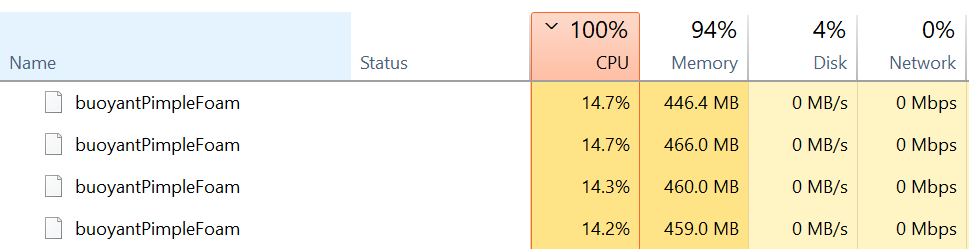
\includegraphics[width=6.27in,height=1.61in]{./media/image23.png}
	\end{Center}
\end{figure}


%%%%%%%%%%%%%%%%%%%% Figure/Image No: 12 Ends here %%%%%%%%%%%%%%%%%%%%

\par

Needs this much RAM  1.6 GB.\par

So 1 million cells to about 1.6 GB ram is to be expected\par

\paragraph{Can i change how we decomposePar our domain for a Speed Tweak? (not quite)}\par



One small tweak with parallel processing, I will split in x and z direction instead of y direction.\par

Original:\par



%%%%%%%%%%%%%%%%%%%% Figure/Image No: 13 starts here %%%%%%%%%%%%%%%%%%%%

\begin{figure}[H]
	\begin{Center}
		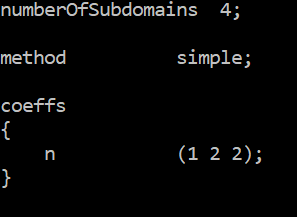
\includegraphics[width=3.09in,height=2.26in]{./media/image24.png}
	\end{Center}
\end{figure}


%%%%%%%%%%%%%%%%%%%% Figure/Image No: 13 Ends here %%%%%%%%%%%%%%%%%%%%

\par

For DNS test 3.2 million cells, 1 parallel timestep calculation with y and z split in 2 and 2 costs $ \sim $ 60s.\par

I can change the setting to this\par



%%%%%%%%%%%%%%%%%%%% Figure/Image No: 14 starts here %%%%%%%%%%%%%%%%%%%%

\begin{figure}[H]
	\begin{Center}
		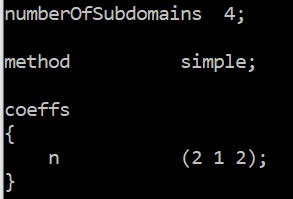
\includegraphics[width=3.05in,height=2.07in]{./media/image25.png}
	\end{Center}
\end{figure}


%%%%%%%%%%%%%%%%%%%% Figure/Image No: 14 Ends here %%%%%%%%%%%%%%%%%%%%

\par

The area of cells talking to each other so to speak diminishes$ \ldots $  (I hope)\par

Okay regardless how its split here, computation time is roughly the same.\par


\vspace{\baselineskip}
\uline{Back to main topic of Batchelor scales}\par

My Alternative is to convert my current case into an air case with same temperature bounds. Though likely that will change the Grashof and Rayleigh number quite a bit. \par

\vspace{\baselineskip}
My case is blowing up. If it’s truly a batchelor scale issue, I can try decreasing the turbulent Prandtl number to increase the turbulent conduction. That’s one way to deal with it.\par

Turbulent Prandtl number decrease to 1e-5.\par

This significantly increases  \(  \alpha _{t} \)  which should simulate the extra large   \( \overline{v'T'} \)  interactions as compared to   \( \overline{u^{'}v^{'}} \) \par

Okay im still getting a blowup here$ \ldots $  I wonder why.\par

But if  \(  \nu _{sgs} \rightarrow 0 \) , doesn’t matter how big  \(  \alpha _{t} \)  will be, there will still be big convection fluctuations generated. Very hard to model.\par


\vspace{\baselineskip}
One thing I catch however, is that ubar is positive (flow is moving up!)\par

Ubar should be negative, and that is same with downcomer. \par

However, when case blows up, uncorrected ubar goes from 0.224 to about -1e7. Which means there is a natural convection downwards, that’s the only thing that can cause this.\par

So definitely problem is with natural convection.\par
\begin{itemize}
	\item If the problem is \uline{only} with natural convection then id say take out the temperature differences.\par

	\item However, it seems that pimpleFoam has a problem with small mesh sizes in general. Not just buoyantPimpleFoam. So doubtfully it’s just natural convection.\par
\end{itemize}

\section{IDDES Run 4, Trying things out with air as the fluid to make Kolmogorov scales the smallest Relevant Scales}

\uline{Imitation with air  takes out the Batchelor Scale problem, plus there are profiles to compare to}\par

Let me simulate with air and see if anything changes.\par

I’ll use the same Reynold’s number.\par

Looks like Openfoam is quite ill-equipped to simulate high Pr fluids in turbulent motion! (I don’t really know, pimplefoam also has some problems in general)\par

Let’s try imitating one case for air, then call it a day  don’t think that’s feasible but can try first at least\par

The Pr is 0.705,  \(  \mu =1.805\ast10^{-5}~ \) \par

At 70C, air kinematic viscosity is  \(  \approx 2e-5 \) \par

\href{https://www.engineersedge.com/physics/viscosity_of_air_dynamic_and_kinematic_14483.htm}{https://www.engineersedge.com/physics/viscosity\_of\_air\_dynamic\_and\_kinematic\_14483.htm$\#$ :$ \sim $ :text=The$\%$ 20viscosity$\%$ 20of$\%$ 20air$\%$ 20depends,2$\%$ 20$\%$ 2Fs$\%$ 20or$\%$ 2014.8$\%$ 20cSt.}\par

To keep Re=2350\par

 \[ 2350=\frac{u \left( 0.015 \right) }{2e-5 } \] \par

 \[ u_{mean}=2350\ast\frac{2e-5}{0.015}=3.133\frac{m}{s} \] \par

My alternative is to make the width bigger, though that will increase the grashof number\par


\vspace{\baselineskip}
\href{http://www.thermopedia.com/content/1191/}{http://www.thermopedia.com/content/1191/}\par

(im testing solver stability first rather than compare cases)\par

 \[  \beta _{IdealGas}=\frac{1}{T \left( K \right) } \] \par

 \[ Gr=\frac{g \beta  \Delta TL^{3}}{ \nu ^{2}}=\frac{9.81 \left( \frac{ \Delta T}{T} \right)  \left( \frac{0.015}{2}^{3} \right) }{2e-5} \] \par

 \[ Gr=\frac{g \beta  \Delta TL^{3}}{ \nu ^{2}}=\frac{9.81 \left( \frac{40}{70} \right)  \left( \frac{0.015}{2} \right) ^{3}}{ \left( 2e-5 \right) ^{2}}=5912 \] \par

Let me increase L to match Gr\par

The number to match is 95567\par

 \[ Gr=\frac{g \beta  \Delta TL^{3}}{ \nu ^{2}}=\frac{9.81 \left( \frac{40}{70} \right)  \left( \frac{H}{2} \right) ^{3}}{ \left( 2e-5 \right) ^{2}}=95567 \] \par

Only thing I want to match here is Kolmogorov scale resolution, other quantities don’t have to match\par

Using solver\par

 \[ \frac{H}{2}=0.01896 \] \par

 \[ H=0.03793 m \] \par

Therefore,  \( u_{mean} \)  needs to be:\par

 \[ u_{mean}=2350\ast\frac{2e-5}{0.03793}=1.23924\frac{m}{s} \] \par

This way I match Re and Gr\par

An easy hack is to change the length scale in blockMeshDictIDDES\par

 \[ scale=0.01\ast\frac{0.03793}{0.015}=0.02528 \] \par


\subsubsection{I noticed that i forgot to turn on my LES model, but even turning it back on don't matter}
\uline{What about my LES model??}\par

One thing I noted, my LES model was turned off! For the previous runs\par

Let me test the LES mesh with LES model on before I do something else eg. air.\par

Setting blockMesh back to 36$\ast$ 158$\ast$ 36\par

And courant number back to 0.5.\par


\vspace{\baselineskip}
Anyhow looks like model blowing up again.\par

\subsubsection{Is the issue again that a bad initial field was given?}

Regardless if I start from T=200 or T=0, blows up!\par


\subsubsection{The air test has failed, so insufficiently resolving scales is not the issue}
But now let me try the alpha stability test again. That failed.\par

Note that bounding omega has exponentially increased: max 7.19e28\par


\vspace{\baselineskip}

\subsubsection{I suspect again it may be a case where the initial field is too far from steady state, thus the solver blows up}
\paragraph{maybe boxTurb can help us generate good initial fields}
\uline{boxTurb for initial field???}\par

Anyhow, if turbulence doesn’t seem to be doing anything, maybe I’ll try boxTurb to start a $``$good$"$  initial field??\par

\subsection{I suspect that pimpleFoam in general isn't too well suited for resolving turbulence, LES or DNS, but it runs ok with RANS type!}



\uline{So how unstable is pimpleFoam and how can we get it to stabilise?}\par

I don’t really know anymore$ \ldots $  but we can look at some cases with fine meshes where pimpleFoam doesn’t blow up\par


\subsubsection{There may be some hope with pimpleFoam, ie take heat transfer out of the equation}

Three cases with LES fine mesh:\par

\href{https://www.openfoam.com/documentation/guides/latest/doc/verification-validation-turbulent-periodic-hill.html}{https://www.openfoam.com/documentation/guides/latest/doc/verification-validation-turbulent-periodic-hill.html}\par

\href{https://www.openfoam.com/documentation/guides/latest/doc/verification-validation-turbulent-plane-channel-flow.html}{https://www.openfoam.com/documentation/guides/latest/doc/verification-validation-turbulent-plane-channel-flow.html}\par

\href{https://www.openfoam.com/documentation/guides/latest/doc/verification-validation-turbulent-surface-mounted-cube.html}{https://www.openfoam.com/documentation/guides/latest/doc/verification-validation-turbulent-surface-mounted-cube.html}\par

Apparently channel flow is possible with mesh$ \ldots $ \par

 \[  \Delta x^{+}=49.6,~  \Delta z^{+} \approx 15.1,~  \Delta y^{+} \approx 1.1 \] \par

Now this is LES for sure. I’d of course like to see if  \(  \Delta x^{+} \)  can drop below 40$ \ldots $  this is critical.\par

 \par

Note that this channel flow has about 1.8-2.4 million cells, which is pretty high.\par

And they do with 8 processors$ \ldots $  wow.\par

To run:\par

Mpirun -np 8 pimpleFoam -parallel $\&$ \par


\vspace{\baselineskip}
Interesting, more than 2 pimple iterations are used.\par
\begin{itemize}
	\item Outercorrectors used 3 times\par

	\item nCorrectors used 1 time\par
\end{itemize}


Courant number is about 1.3-1.4\par

If that floats the boat, that floats the boat, it’s not 5 or 10$ \ldots $ \par


\vspace{\baselineskip}
Note this also, the pimple solver uses only the final settings so to speak$ \ldots $  (in the fvSolutions),\par

I’m not using the full capability!\par


\vspace{\baselineskip}
\subsection{pimpleFoam Plane Channel Flow test Results, LES mesh size $\Delta x^{+}=40$ with kEqn in pimpleFoam is ok}\par
Plane channel flow in the OpenFoam tutorials was modified to give a smaller mesh. Such that  \(  \Delta x^{+} \)  can drop below 40. (I made 625 grid points in blockMesh rather than 500)\par

However, the BCs are different here and so is the solver.\par

The solver here is pimpleFoam\par



\begin{itemize}
	\item no cyclic conditions are used for inlet/outlet, instead a turbulentDFSEM intlet is used to artificially generate eddies\par

	\item a fixed outlet pressure is also used\par
	
	\item \href{https://www.openfoam.com/documentation/guides/latest/doc/verification-validation-turbulent-plane-channel-flow.html}{https://www.openfoam.com/documentation/guides/latest/doc/verification-validation-turbulent-plane-channel-flow.html}\par


\end{itemize}
The simulation run is \uline{very} stable, runs for 30-65s without any flaws. \par

\begin{itemize}
	\item Started 0-31s with timestep 0.004, CFL$ \sim $ 1.2 (constant)\par

	\item From 31s-63.5s, set maxCo=0.5\par

\begin{itemize}
	\item Max CFL will fluctuate periodically, which should be expected for resolved eddies\par

	\item Timestep will adjust to make max Co set at 0.5\par

	\item Oscillations are manageable, solver does not blow up after this set time (don’t know if it will in long run, ie 100s of seconds, but I doubt we need to measure time for that long)\par

Solver has completed running after about 2 weeks at 8 processes. \par

Oscillations manageable, not solver blow up, stable performance with adjustable timestep. So it goes to show with the right settings, resolution of turbulence is still possible.\par

\end{itemize}
\end{itemize}

\section{IDDES Run 5: IsoThermal BuoyantPimpleFoam}\par

\subsubsection{i suspect heat transfer may cause the instability issue, thus i'm trying buoyantPimpleFoam but making the entire case isothermal}
Can similar stability be done for buoyantPimpleFoam?\par

I suppose so, \uline{I want to eliminate natural convection as cause of instability} so I’m just switching to isothermal BCs for buoyantPimpleFoam, to test if the solver itself has capability to handle the small mesh.\par

However, I ran buoyantPimpleFoam copying IDDESCase2 and changing temp BCs to isothermal, and the solver crashed due to exponential CFL number.\par

I then tried using a RANS type mesh and ran the same thing, again it crashed. \par

I wonder what mistake I made there$ \ldots $  did I change fvSchemes or some other thing to cause instability?\par

I’m re-running the RANSCase1 which worked before as a test.\par

In fact IDDESCase1 also worked which I can then use for a template for IDDESIsothermal (which is IDDES model used with isothermal BCs).\par


\vspace{\baselineskip}
The RANS case is quite stable. So I’m quite satisfied.\par

I hope the isothermal BC is not causing system crash.\par

To organise which cases are stable and which are unstable, \par

I should rename RANSCase1 and IDDESCase1 as stable cases, unproven cases are called test cases.\par


\vspace{\baselineskip}
\section{IDDES Run 6: Removing cyclic BCs as a cause of instability}\par

One other reason for instability is inappropriate BCs. \par

Instability has many reasons, a smaller mesh size in openfoam tends to be more numerically unstable as numerical errors may make up a larger percentage of the simulated data. (conjecture)\par

Any simulation with stiff type BCs can cause this to happen. There must be a way to dampen these data out\par


\begin{itemize}


	\item One is via larger mesh size\par

	\item Second is via stable BCs\par
\end{itemize}
Taking large mesh size away as a way to dampen the errors may leave the error dampening mechanisms insufficient.\par

Probably need more error dampening mechanisms:\par



\subsubsection{What constitutes Stable BCs?} \par

\begin{itemize}
	\item eg pressure must be fixed at one end, rather than left as a cyclic patch\par

\begin{itemize}
	\item better yet have a fixed pressure drop and zerogradient velocity\par


\end{itemize}
	\item velocity should be fixed at one end and zerogradient at the other\par

	\item Refer to this table:\par

\begin{itemize}
	\item \href{https://www.openfoam.com/documentation/guides/latest/doc/guide-bcs-common-combinations.html}{https://www.openfoam.com/documentation/guides/latest/doc/guide-bcs-common-combinations.html}\par

	\item \href{https://cfd.direct/openfoam/user-guide/v7-boundaries/}{https://cfd.direct/openfoam/user-guide/v7-boundaries/}\par
	\item A larger library of stable tutorial cases!\par


\end{itemize}
\end{itemize}

\begin{itemize}
	\item \href{https://cfd.fossee.in/case-study-project/case-study-run/20}{https://cfd.fossee.in/case-study-project/case-study-run/20}\par

\end{itemize}

\vspace{\baselineskip}
So if I take away the cyclic BCs, I can instead have a fixed temperature inlet BC, fixed pressure inlet BC, and sort of tune it to get a desired velocity and Re.\par


\vspace{\baselineskip}
This way instead of simulating an infinitely long inlet, I simulate the entrance region, which could be easier to validate.\par

I posit that if the entrance heat trf coeffs and friction can be matched (DNS-LES-RANS), it is at least a second best guestimate for the rest of the flow (infinite periodic region).\par

Alternative is this, \uline{if stable} and the entrance U, T and p fields are developed in LES, then I map these to LES in periodic BC with help of change dictionary. (I can have a entrance region case which is stable and copy into the file)\par


\vspace{\baselineskip}
\paragraph{RANS Case 1 and IDDES Case 1 seems to work well with cyclic BCs!}  \par


What would I wish to work? IDDESCase2\par

How? We’ll want to test IDDES Case 2 type mesh with New BCs first (343k entry temperature, no periodic BCs, zerogradient Exit), what should velocity be? Turbulent DFSEM inlet and zerogradient outlet with correct average velocity$ \ldots $ \par

Apparently fixed mass/vol flowrate and fixed static pressure is very stable in the outlet.\par

\href{https://www.openfoam.com/documentation/guides/latest/doc/guide-bcs-common-combinations.html}{\textcolor[HTML]{0000FF}{\ul{https://www.openfoam.com/documentation/guides/latest/doc/guide-bcs-common-combinations.html}}}\par

\subsubsection{Possible BCs to use}
\vspace{\baselineskip}
The velocity BC can be set as fixed flowrate with ability to extrapolate velocity profile downstream.\par

\href{https://www.openfoam.com/documentation/guides/latest/doc/guide-bcs-inlet-flow-rate-inlet.html}{https://www.openfoam.com/documentation/guides/latest/doc/guide-bcs-inlet-flow-rate-inlet.html}\par



DFSEM inlet can also be used for turbulence generation. Necessary? Not sure$ \ldots $  but definitely more physical.\par

To see if its stable.\par



%%%%%%%%%%%%%%%%%%%% Figure/Image No: 15 starts here %%%%%%%%%%%%%%%%%%%%

\begin{figure}[H]
	\begin{Center}
		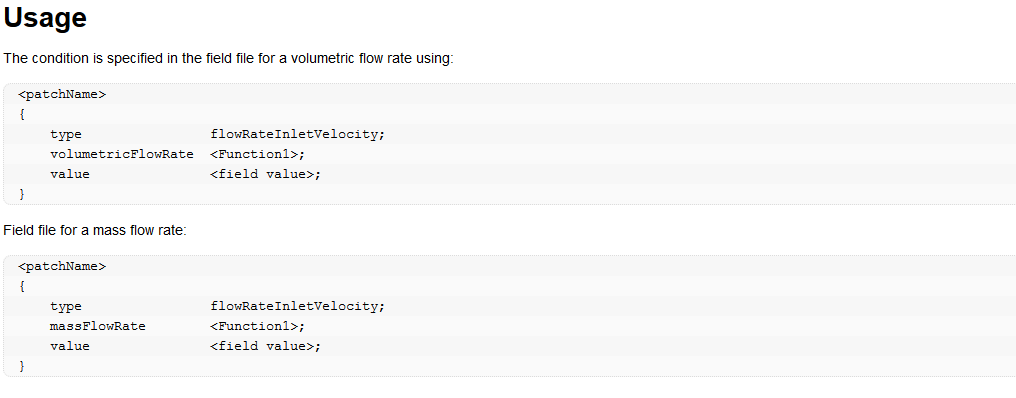
\includegraphics[width=6.27in,height=2.46in]{./media/image26.png}
	\end{Center}
\end{figure}


%%%%%%%%%%%%%%%%%%%% Figure/Image No: 15 Ends here %%%%%%%%%%%%%%%%%%%%

\par

Hopefully this will be stable$ \ldots $ \par

Velocity of 0.22618 m/s gives Re$ \sim $ 2350. So I’ll put this into my BCs.\par


\subsubsection{Steps taken to change BCs}
Here are the steps taken:\par

\paragraph{BlockMesh}
 Changed inletoutlet into patch in blockMeshDictIDDES\par

\subparagraph{Rename the patches because I got my inlet/outlet and side periodic patches mixed up} \par


Seems I’ve been simulating the wrong thing all along LOL\par

 Nevertheless it shows that it can work for smaller cases\par

 I’d like to see it work for larger cases though\par

 Next time place the x and y and z coordinates of the planes in blockmesh for easier refernce\par

 But anyhow for cyclic conditions, it doesn’t really matter how I name the patches, only wall is impt as well as temperature of plate  physically still simulating correct thing but wrong patch names that’s all \par


\paragraph{changeDictionary}


Change BCs using changeDictionary\par

\subparagraph{Velocity inlet and outlet}


For velocity, inletoutlet and turbulentDFSEM is used\par

\subparagraph{Pressire BCs} \par



Pressure
\begin{enumerate}
	\item Cyclic at cyclic BCs\par

	\item Calculated otherwise\par
\end{enumerate}

P\_rgh\par

\begin{enumerate}
	\item Inlet zerogradient (or for this case, since its compressible we use fixedfluxpressure)\par

\begin{enumerate}
	\item \href{https://cfd.direct/openfoam/user-guide/v6-boundaries/}{https://cfd.direct/openfoam/user-guide/v6-boundaries/}  \par


\end{enumerate}
	\item Outlet will be fixed value\par

\end{enumerate}

\subparagraph{Temperature BCs}


For temperature, inlet is 343K, outlet is also fixed to 343K\par


\subparagraph{Turbulence Quantities BCs}



For k $\&$  omega \par



\begin{enumerate}
	\item \href{https://www.researchgate.net/post/How_do_we_give_boundary_conditions_in_k_omega_SST_model_for_airfoil_simulation_in_OpenFOAM}{https://www.researchgate.net/post/How\_do\_we\_give\_boundary\_conditions\_in\_k\_omega\_SST\_model\_for\_airfoil\_simulation\_in\_OpenFOAM}\par

	\item Can expect low level or turbulence to be modelled,\par

\begin{enumerate}
	\item For 5$\%$  intensity, I can expect 20$\%$  to be modelled for typical LES\par

	\item Hence turbulent intensity can set to 1$\%$ \par

	\item In the turbulentDFSEM case, a miniscule value is used for k (1e-5)\par

\begin{enumerate}
	\item \href{https://develop.openfoam.com/Development/openfoam/-/blob/master/tutorials/incompressible/pimpleFoam/LES/channel395DFSEM/0/k}{https://develop.openfoam.com/Development/openfoam/-/blob/master/tutorials/incompressible/pimpleFoam/LES/channel395DFSEM/0/k}\par

	\item Outlet is inletOutlet (zerogradient for outflow, fixedvalue for reverse flow) with $\$$ internalField as value\par


\end{enumerate}
	\item For omega I can set it to count on mixing length $ \sim $  l= 0.038$\ast$ d\textsubscript{h}\par

\begin{enumerate}
	\item Or 0.038 channel width \par

	\item \href{https://www.cfd-online.com/Forums/openfoam-solving/185059-k-omega-inlet-k-omega-sst.html}{https://www.cfd-online.com/Forums/openfoam-solving/185059-k-omega-inlet-k-omega-sst.html}\par

	\item I used 7$\%$  channel width for simplicity\par

	\item Outlet is inletOutlet, fixed reverse flow revalue and initial value with $\$$ internalField as value\par


\end{enumerate}
	\item For nut \par

\begin{enumerate}
	\item I set it to zerogradient/nutUWallFunction at walls\par

	\item Cyclic at cyclic boundaries\par

	\item Calculated with initial value of 1e-8 (similar to the channel395 DFSEM values)\par


\end{enumerate}
	\item For epsilon (if I ever use it)\par

\begin{enumerate}
	\item \href{https://www.openfoam.com/documentation/guides/latest/doc/guide-bcs-inlet-turbulent-epsilon-turbulent-mixing-length-dissipation-rate.html}{https://www.openfoam.com/documentation/guides/latest/doc/guide-bcs-inlet-turbulent-epsilon-turbulent-mixing-length-dissipation-rate.html}\par

	\item For inlet outlet turbulent mixing length dissipation rate (0.07 times channel width)\par


\end{enumerate}
	\item Alphat\par

\begin{enumerate}
	\item Wallfunctions with Prt of 0.85\par

	\item Initial condition of 0, (doesn’t seem physical however)\par

\begin{enumerate}
	\item But usually code will calculate it using a Prt\par


\end{enumerate}
	\item Inlet and outlet done using calculated\par

	\item \href{https://develop.openfoam.com/Development/openfoam/-/blob/master/tutorials/heatTransfer/buoyantSimpleFoam/circuitBoardCooling/0.orig/alphat}{https://develop.openfoam.com/Development/openfoam/-/blob/master/tutorials/heatTransfer/buoyantSimpleFoam/circuitBoardCooling/0.orig/alphat}
\end{enumerate}
\end{enumerate}
\end{enumerate}\par
\subsubsection{Getting TurbulentDFSEMInlet to Work Right}
debug log\par

round 1 says that there is some error, likely syntax or something, or missing tensor value,\par

I suspect turbulent DFSEM doesn’t have an initial field to start, which is why is fails.\par

I tested the code by commenting out portions of the code one at a time. Sure enough it’s in the turbulentDFSEM part\par

I notice the header file of for DFSEM case channel395DFSEM says location 1 $ \ldots $  why?\par


\vspace{\baselineskip}
Oh I found the bug, we need patch values for R, U and L, the Reynolds stress tensor\par

\href{https://www.openfoam.com/releases/openfoam-v1606+/boundary-conditions.php}{https://www.openfoam.com/releases/openfoam-v1606+/boundary-conditions.php}\par

these should be in the constant directory.\par

Okay. So based on these tensors we simulate turbulence.\par

Useful article:\par

\href{http://www.tfd.chalmers.se/~hani/kurser/OS_CFD_2012/NinaGallJorgensen/ReportReviewed.pdf}{http://www.tfd.chalmers.se/$ \sim $ hani/kurser/OS\_CFD\_2012/NinaGallJorgensen/ReportReviewed.pdf}\par


\vspace{\baselineskip}
In general timevaryingMappedFixedValue should be able to work as well, almost like a semi periodic BC.\par

In pisoFoam pitzDailyMapped there is such a BC.\par

It is also known as mapped in the ESI release of OpenFoam.\par

Anyhow to obtain boundary data, probably need to use some postprocessing to obtain the relevant length scales, U fields, reynold’s stress tensor and points file.\par

\textbf{How to generate these fields?}\par

Reynold’s stress field can be obtained using\par

buoyantPimpleFoam -postProcess -func R\par

\href{https://cfd.direct/openfoam/user-guide/v6-post-processing-cli/}{https://cfd.direct/openfoam/user-guide/v6-post-processing-cli/}\par

the other way is using boundaryData$ \ldots $ \par

\href{https://www.openfoam.com/releases/openfoam-v1606+/boundary-conditions.php}{https://www.openfoam.com/releases/openfoam-v1606+/boundary-conditions.php}\par

so basically its sampling using functionObjects and releasing it as boundaryData format$ \ldots $ \par

\href{https://www.openfoam.com/documentation/user-guide/userse21.php}{https://www.openfoam.com/documentation/user-guide/userse21.php}\par

Okay$ \ldots $  can do after lunch. \par

I can specify some random values first for turbulentDFSEM.\par

Just want to test stability.\par

Using this format$ \ldots $ \par

inlet \\
$ \{ $  \\
    type        turbulentDFSEMInlet; \\
    delta       2; \\
    R           uniform (xx xy xz yy yz zz); \\
    U           uniform (x y z); \\
    L           uniform x; \\
    value       (0 0 0); \\
$ \} $ \par

Oh boy it works! (the BC does anyway)\par

Okay testing on big mesh, no exceptionally large Courant numbers$ \ldots $ \par

($ \sim $ 200,000 cells simulation)\par

Doesn’t seem to blow up yet though. (t=0.07s)\par

Looks like non periodic does make the simulation stable. So correct BC setting is impt. Esp for LES where stabilising effect of large timestep is removed. Likewise looks like DNS requires the same things to work.\par

Running parallel on this mesh$ \ldots $ \par

So looks good! Solver is stable at these times. (t=2.31 s), (t=5.21s)\par

How then do I get data\par

I even left the fvOptions for mean flow on by accident and that still doesn’t affect stability much!\par


\vspace{\baselineskip}
I can use the turbulenceFields function to calculate R and L. \par

So I can get a snapshot of U, R and L at some specified points. Great! I can then map these over to boundary field data (just remember that the patch names may be different cos I named them wrongly)\par

Oh man, I also forgot, i made the flow in the wrong direction! Got to run the RANS and IDDES case again$ \ldots $ \par

Let’s mend the git repository and pull changes in.\par


\vspace{\baselineskip}
Btw, for large files more than 100MB or more, one can actually decomposePar to make them become less than 100 MB then it makes it easy to upload on github.\par
\begin{itemize}
	\item I first uploaded the pimpleFoam files directly to github (turbulentDFSEMInlet files after running stably for 85s and cleaning it out)\par

	\item I pushed the commits from the IDDES branch and merged it into the master branch, thus resolving the problem$ \ldots $ 
\end{itemize}

\par

\subsubsection{Generating R, L and U boundaryData for turbulentDFSEMInlet}

\uline{The function Object branch}\par

Now I want to include function objects, so i’m making a branch for function objects.\par

\href{https://www.openfoam.com/documentation/guides/latest/api/classFoam_1_1functionObjects_1_1turbulenceFields.html}{https://www.openfoam.com/documentation/guides/latest/api/classFoam\_1\_1functionObjects\_1\_1turbulenceFields.html}\par

Firstly I’ll want to generate turbulence fields\par

And I’ll also want to write the coordinates into a points file so that the boundaryData format.\par

For easy reference, this may help.\par

\href{https://www.openfoam.com/documentation/user-guide/userse21.php}{https://www.openfoam.com/documentation/user-guide/userse21.php}\par

I already have a sets function:\par



%%%%%%%%%%%%%%%%%%%% Figure/Image No: 16 starts here %%%%%%%%%%%%%%%%%%%%

\begin{figure}[H]
	\begin{Center}
		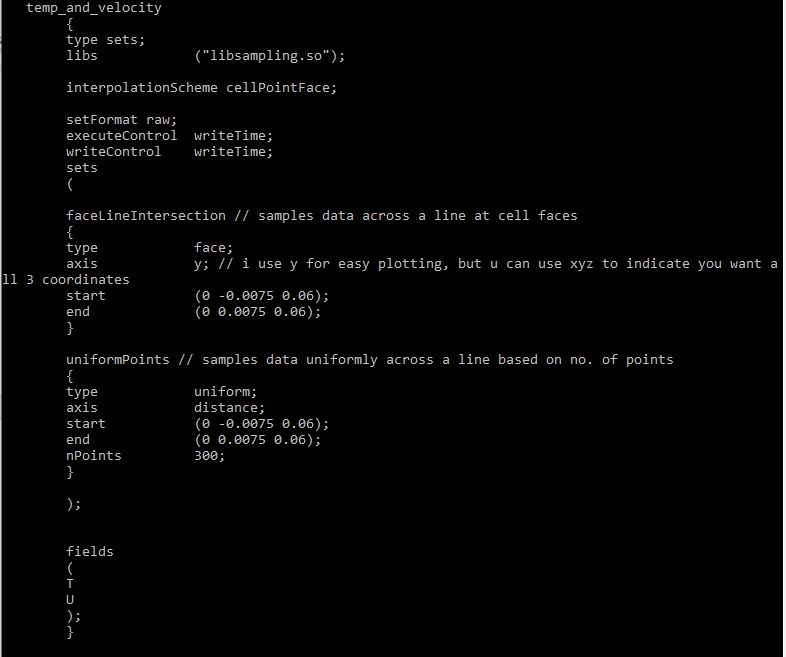
\includegraphics[width=3.51in,height=2.94in]{./media/image27.png}
	\end{Center}
\end{figure}


%%%%%%%%%%%%%%%%%%%% Figure/Image No: 16 Ends here %%%%%%%%%%%%%%%%%%%%

\par

A similar thing should be used to write boundaryData.\par

I can include this in controlDict and runFunctionObjects.\par


\vspace{\baselineskip}
\begin{itemize}
	\item Let me just try doing boundaryData of velocity.\par

	\item \href{https://www.openfoam.com/documentation/guides/latest/doc/guide-fos-sampling-surfaces.html}{https://www.openfoam.com/documentation/guides/latest/doc/guide-fos-sampling-surfaces.html}\par

	\item this is the correct function object for sampling surface data.\par


\vspace{\baselineskip}
	\item An example of use is found here:\par

	\item \href{https://develop.openfoam.com/Development/openfoam/-/blob/master/tutorials/incompressible/pimpleFoam/RAS/propeller/system/surfaces}{https://develop.openfoam.com/Development/openfoam/-/blob/master/tutorials/incompressible/pimpleFoam/RAS/propeller/system/surfaces}
\end{itemize}\par


\vspace{\baselineskip}
use buoyantPimpleFoam -postProcess\par

to start the postprocess functions.\par

So after some debugging, I get the correct syntax and this works, T and U are on the patches, but somehow the temperature is uniform on the patch (strange!).\par

At least the code syntax is right.\par

Argh so annoying, my changes were undone..\par



%%%%%%%%%%%%%%%%%%%% Figure/Image No: 17 starts here %%%%%%%%%%%%%%%%%%%%

\begin{figure}[H]
	\begin{Center}
		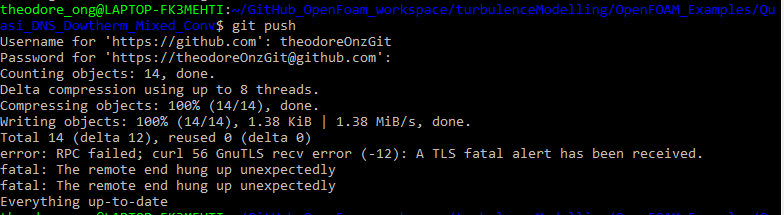
\includegraphics[width=6.27in,height=1.72in]{./media/image28.png}
	\end{Center}
\end{figure}


%%%%%%%%%%%%%%%%%%%% Figure/Image No: 17 Ends here %%%%%%%%%%%%%%%%%%%%

\par

\paragraph{Windows Subsystem for Linux 2 Github bug in Jun 2020}

And I cannot push my changes up to github$ \ldots $  I wonder why.\par

There is a possibility the remote hangup is due to a WSL2 error.\par

I thought it was due to size and so I uploaded leaner versions of the file to a new repo (turbulenceModelling2)\par

Even when I ran ./Allclean on pretty much everything there, the same error came up.\par

I’m trying this on linuxMint to see if it gives me the same issue.\par

linuxMint gives me an upload even with large files and after cleaning up all the commit history IT’S OK.\par

I’m suspectin it’s a WSL 2 problem, so bye bye WSL 2..\par


\vspace{\baselineskip}
WSL works perfectly for such issues, no problem there.\par
\paragraph{In case my Boundary Conditions weren't Correct...}
\uline{Resetting BCs for the original case}?\par

I didn’t do the names of the blockMesh right, I thought that means that the flow will be like such:\par



%%%%%%%%%%%%%%%%%%%% Figure/Image No: 18 starts here %%%%%%%%%%%%%%%%%%%%

\begin{figure}[H]
	\begin{Center}
		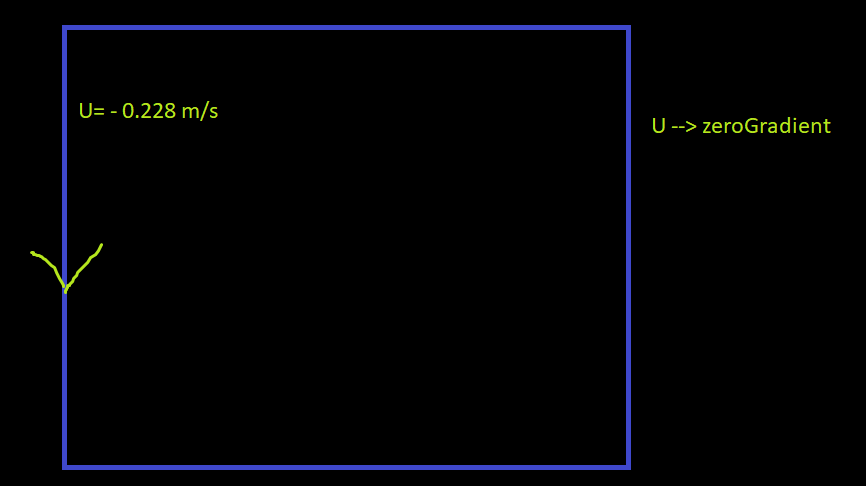
\includegraphics[width=6.26in,height=3.51in]{./media/image29.png}
	\end{Center}
\end{figure}


%%%%%%%%%%%%%%%%%%%% Figure/Image No: 18 Ends here %%%%%%%%%%%%%%%%%%%%

 But this is not the case. \par

How I name the BCs has marginal impact on the flow since I use a forcing function for the flow$ \ldots $  and the conditions are cyclic anyhow. The only impact is this: that the mesh sizing spanwise and streamwise will be different.\par

Shouldn’t be an issue now though$ \ldots $ \par


\vspace{\baselineskip}

\par


So i have found a way to place boundary data in surface format from
existing fields, eg. T U on my github. 

Repo is here: https://github.com/theodoreOnzGit/turbulenceModelling.git.

Now I actually want to have my data as including turbulent quantities
for the inlet fields. Now, this will actually calculate all relevant
fields, eg. k, epsilon, omega, R (Reynold's stress tensor), L (mixing
length), I (turbulence intensity), nuTilda (spalart allmaras variable).
This enables my field from k-omega SST IDDES to be applied also to
SA-IDDES fields. That's pretty good!

In addition i can map alphat as well, which should prove useful. For
heat transfer, but maybe that part I'll do later. Thankfully the entry
is well documented!

\paragraph{Interpolation causes issues with TurbulentDFSEMInlet}

Now i'm getting an error: my fields read right but when some values
of reynold's stress tensor are less than 0 (indicative of backscatter). 

What i notice though about the fields is that the values close to
0 are often minute ($10^{-6}$) whereas the positive values are on
the order $10^{-4}$. The idea is to replace all the negative values
with 0. Using the sed fucntion sed 

-i ``s/-{*}/0/g'' <filename> 

to replace all the negative values. Unfortunately, the values themselves
are in scientific format eg. e-07. So i'll need to instead use 

sed -i ``s/-1.{*}/0/g'' <filename> 

in order to replace all the relevant data points.

Furthermore, sed actually replaces following the --1.{*} with 0,
including all following numbers!

Doesn't look like sed makes it easy!

Another way to approach: use the RANS mesh case. (unfortunately that
too has negative numbers)

So got to use sed

The way is this: 

URL reference: https://www.unix.com/unix-for-dummies-questions-and-answers/246213-sed-awk-find-negative-numbers-replace-1-a.html

sed ``s/-{[}0-9{]}.{[}0-9{]}{*}/0/g'' <filename>

unfortunately that also replaces all the powers with e-09 to e0. Placing
one more specifier works!

sed ``s/-{[}0-9{]}.{[}0-9{]}{[}0-9{]}{*}/0/g'' <filename>

Ayio, again sed does not like R\_xx=0, it must be >0. 

Also to have better control of values replaced by spacebar, one can
use 

sed -i 's/0 /1e-09 /g' <filename>

to do replace specific value

Looks like i mseed it up but, then again i look at the R file, only
one value in R\_XX is negative, may as well change that.

Looks like that solved it! Must have been some interpolation error.
Only face 76 seems to be an issue

Can i interpolate such that it doesn't give me this issue?

Or i can make interpolate false!

That should debug things. 

After debugging, interpolate false works, the fields can now be read.
But issue is that again i have the IOStream error....

ima try to leave out the nCellsPerEddy case...

Doesn't work... ugh.

Can check turbulentDFSEMInlet Source code to see the correct input
mode:

https://www.openfoam.com/documentation/guides/latest/api/classFoam\_1\_1turbulentDFSEMInletFvPatchVectorField.html

im still not really sure, but let erase the first line: value 1264
from points, and that should be ok. (doesn't really make a diff whether
u have it or not)

Done this and still gives the error (error in IOstream)

Looks like the points on the right side BC were missing!

now everything works well. the simulation is running without stability
issues

I also want to map pressure and temperature fields as well as alphat
type fields and nut type fields if possible.

\subsubsection{Results of IDDES Run 6}
syntax is ok but courant Number still blows up =(

Probably does so on injected turbulence.

The other time i did the entrance BC, it was stable probably because
turbulence structures were not well formed yet. 

However, it was stable till 0.1595s.

My other option is to increase the corrections in my pimple loop.
(ie give it more outercorrectors)

Okay even that crashed, but it crashed much faster though! (within
one calculation it crashed)

This may give some interesting insight.

(but i'll leave it for later, in another section)

The trend is a steadily increasing maxCo, for which the timestep adjusts
to compensate to make maxCo about 0.5. At timestep = 7e-05 timestep
decreases steadily. At about timestep adjusted to 5.5e-05, the iterations
get more and more long to calculate, lag is noticeable. 

At timestep below 5e-05, oscillations increase rapidly. Solver instability
happens. Why this number though and not other numbers...

The mean Co also starts to jump exponentially at timestep below 5e-05. 

Can look here for examples:

https://cfd.fossee.in/case-study-project/case-study-run/20

\section{IDDES Run 7: Switching off Natural Convection}

This is just conjecture, but since the pimpleFoam case works, i suspect
buoyantPimpleFoam will work without gravity.



Funny though, even without gravity the solver is facing the same issues.



Apparently it's the maxCo which is driving the timestep ultrasmall
to keep maxCo at 0.5, the mean Co actually remains relatively small
0.016 ish. So at around 0.159727s again, it fails. Even without natural
convection. So it's a problem then with resolving the forced convection
bit more like. Natural convection does not play too much of a role
in these instabilities. 



\section{IDDES Run 8: (not done)}



channel395DFSEMInlet case uses kEqn, i use kOmegaSSTIDDES. While kEqn
resolves turb BL, kOmegaSSTIDDES will have a RANS region gradually
transitioning to LES region.



Could the turbulence model be the issue? I suspect not, even with no turbulence model, the buoyantPimpleFoam Solver Crashes.


I suppose i can switch the model to kEqn and Spalart Allmaras IDDES and see what happens... But i'm taking off from turbulence modelling for now. 

\section{IDDES Run 9: switching from buoyantPimpleFoam to buoyantBousinesqPimpleFoam (also not done)}


I think i recall reading somewhere that buoyantBousinesqPimpleFoam is used for DNS or LES type simulations before. 


I can't quite remember where, but I remember being reluctant to use it because of the bousinesq approximation not being able to fully simulate compressible flows.


However, that now becomes irrelevant since the flows themselves are not compressible anyhow.


A few observations of note:


\begin{itemize}
	\item First that pimpleFoam can resolve LES turbulence well
	\item Second that fireFoam can resolve turbulence LES style
	\item Third, that buoyantPimpleFoam cannot resolve LES turbulence well due to solver instability regardless of gravity on or off, BC change, fvSolutions/fvSchemes tweaking
	
\end{itemize}


I have a conjecture that looking into the buoyantBousinesqPimpleFoam lead may help.


It may be useful to see the source code and how each equation U, P and h is solved for each solver.


But that for another time, I need a break from this problem. 

Okay I tried buoyantBoussinesqPimpleFoam because i needed buoyantPimpleFoam to simulate turbulence on more complex geometries and it was failing badly. 

The mesh was 36*158*36. 

There were some promising results, the max courant number was 2x that of the mean courant number even until crash. The simulation crashed at around 0.06s. But the courant numbers were stable. 


Why was this promising? Well, the background is this: temperature, pressure (mass balance) and velocity are all linked in the solver of buoyantPimpleFoam. Now when an error or local fluctuation in pressure gets too high, buoyantPimpleFoam starts to get wonky. So usually high pressure means results in high velocity, so Courant Numbers explode. Now, in compressible fluids, temperature is linked to density and pressure. So an error in temperature variations can also cause velocity and pressure to become wonky. Thus Courant number explodes and temperature goes negative. 


This is on the whole quite encouraging despite the crash because we did not see courant numbers explode. Only that temperature equation was unable to be solved. And one other note of observation was that the cumulative mass error grew bigger over time.

My suspicion is that for this cyclic case, a decrease in density means that mass has to come in from somewhere and a decrease in density means mass has to go somewhere. However, since this case is cyclic, then the error gets bigger over time. We don't see this in the pimpleFoam channel flow case. So this is one possibility. 

The action is then to make beta 0. And see what happens.


\section{IDDES Run 10: Square Mesh}

One wild conjecture is this, maybe buoyantPimpleFoam does not like skewed meshes to simulate turbulence. Maybe that causes numerical instability, i don't know. 

\subsection{Round 1 of blockMesh 16 million cells (too long)}


But I will want to try a square mesh with 16 million cells. It will be IDDES type of simulation but with symmetrical mesh.


It will be 88 cells in y direction, 264 cells spanwise and 704 cells streamiwise for a total of 16.355 million cells.



Now this ain't too good. BlockMesh itself while on one processor, took a good 20-30 minutes. I'm not too enthusiastic we'll get to the 0.16s threshold before the term ends if each timestep takes like one day, or even 1 minute.

\subsection{Round 2 of blockMesh 8 million cells: okayish}

Let's ease the calculation and give it about 8 million cells:
210*70*560.

This is 70 in the y direction. Where we normally give it about 159 cells in y direction. This is about 2.2 times coarser than $\Delta {y}^{+} = 1$ this means we have $\Delta {y}^{+} \approx  2.2$ in x y and z direction.


Can sort of think of this as coarse mesh DNS. But i don't resolve Batchelor scales.



Note that once list construction is complete of the faces and points (50 million faces mind you), then blockMesh is relatively fast, about 1-2 minutes to complete the process.


Now blockMesh has finished within 5-10 minutes.


Let's now decomposePar using:


mpirun -np 15 redistributePar -decompose -parallel 


Okay that doesn't work



I just used 


decomposePar


and it ran well within 1 minute.



Next i tried doing the simulation


but within 3-4 timesteps, it crashed. Courant number too big.



Back to the drawing board....


I'm closing this investigation for now (02 July 2020).

\section{IDDES Run 11: mapping a coarse $y^+$ mesh to a fine one}

\subsection{blockMesh, getting y+ to 30}

okay so i'm increasing $y^+$ to about 30 ish. This is suitable for RANS near boundary layers. So that's okay for IDDES too. 

Though of course, doing so makes the mesh 14 by 5 by 38 (too coarse).

If i do 30 grids in y direction, $y^+$ is about $5^+$ which is still pretty fine.

I suppose i can do $y^+$=30 for starters.

This case solved in less than 30s, very fast. Or rather, crashed at about 3s of simulation time.
I'm increasing y resolution to 10. 

Simulation seems to crash around 1.8s of simulated time. 

I'm going to introduce relaxation factors to dampen things out. 
Relaxation factor of 0.7 should help do the trick.

Tolerance all round set to 1e-05. Added residual control entries to PIMPLE as well.

Looks like changing fvSolution managed to help increase stability of simulation, made it past 2s.

Simulation is now stable past 3s.
Simulation now stable at 14s with minimal courant disruption, blowups etc.
Time ratio is about 20s of simulated time for 400s of real time (20x). Quite cheap (ran in parallel 4 processors). 

Heat transfer coefficient is about 400-500. 
This is about the same as the RANS simulation which is has about 560 heat transfer coeffcient.

Now stable at 56s. This is a stable case.
About 5320 cells are used. Works almost like a RANS case. 

Ran to 98s, declaring this case stable.

Just not quite steady state yet, the hot side heat trf coeff is more than cold side. 

In fact, after running for 600 plus seconds of simulation time, the heat transfer coefficient for hot side is much greater than that for cold side, and there is a continuity error for mass of about 400 (cumulative). So mass is disappearing and heat. Something is quite wrong.


\section{getting back to IDDES mesh}

now i map these fields to IDDES mesh 40 by 158 by 40. Using pimple loop, residuals do not tend to converge below 0.01. Oscillations are otherwise stable.

I'm changing the initial U residuals to exit at 1e-2 rather than 1e-3.

For speed i'd also change the relaxation factors to 0.9. 

Solver blew up though... 

And relaxation factor at 0.9 doesn't speed it up. It still has the oscillating residual problem.

Relaxation factor 0.5 will also take long.

Not going to waste more time. Closing this investigation.


\vspace{\baselineskip}
\part{Bibliography and Citation}

\printbibliography
\end{document}
